\chapter{Interaction Region Local Coupling Correction in the LHC}
\label{chapter:ir_local_coupling}

The linear optics and coupling correction usually constitute the first phase of machine commissioning as both are major contributors to the performance of colliders, and are required to be under good control for the next phases of commissioning.
In recent years, significant efforts have been made to improve the measurement and correction of linear and non-linear global coupling both in the \gls{LHC}~\cite{PRAB:Tomas:Review_Linear_Optics_Measurements, IPAC:Tomas:Measurement_Coupling_RDTs_LHC_AC_Dipole, PRAB:Calaga:Coupling_Merging_Hamiltonian_Matrix_Approaches, PRAB:Maclean:First_Nonlinear_Errors, PRAB:Maclean:Optics_Commissioning_Nonlinear_Era, PRAB:Persson:Chromatic_Coupling_Correction, PRAB:Tomas:ADECTA, IPAC:Maclean:ADECTA_Octupoles, PRAB:Biancacci:AC_Dipoles_Localize_Sources_Beam_Coupling_Impedance, CERN:Maclean:Demonstration_Coupling_Correction_Below_PerMil_LHC} and other synchrotrons~\cite{PRAB:Tian:Genetic_Algorithms_Storage_Ring, PRAB:Ohnishi:Measurement_Chromatic_XY_Coupling, PRAB:Carla:Local_Transverse_Coupling_Impedance_Measurements_Synchrotron_Light_Source, PRAB:Shen:Application_Independent_Component_Analysis_AC_Dipole_Based_Optics_Measurement_Correction_Relativistic_Heavy_Ion_Collider, PRAB:Sagan:Betatron_Phase_Coupling_Measurements_Cornell_Electron_Positron_Storage_Ring, PRAB:Fischer:Robust_Linear_Coupling_Correction_NTurn_Maps, ARXIV:Franchi:Error_Analysis_Linear_Optics_Measurements_Turn_Turn_Beam_Position_Data_Circular_Accelerators, PRAB:Tomas:Measurement_Local_Global_Resonance_Terms, NIMP:Yang:Method_Simultaneous_Linear_Optics_Coupling_Correction_Storage_Rings_Turn_Turn_Beam_Position_Monitor_Data, NIMP:Xiaobiao:Online_Optimization_Accelerators, IEEE:Raka:Measurement_Linear_Coupling_Brookhaven_AGS, PRAB:Franchi:Vertical_Emittance_Reduction_Preservation_Electron_Storage_Rings_Resonance_Driving_Terms_Correction, NIMP:Aiba:Ultra_Low_Vertical_Emittance_SLS_Systematic_Random_Optimization}, as their effects can lead to instabilities and unwanted dynamics in the machine~\cite{IPAC:Maclean:Effect_Coupling_Nonlinear_Observables, PRAB:Carver:Transverse_Instabilities_With_Coupling, PRAB:Franchi:Emittance_Sharing_Coupling, EPAC:Metral:Destabilising_Effect_Linear_Coupling_HERA_Proton_Ring, PRAB:Biancacci:AC_Dipoles_Localize_Sources_Beam_Coupling_Impedance}.

In the LHC, local coupling correction has so far been done with the Segment-by-Segment technique~\cite{PRAB:Tomas:CERN_LHC_OMC}.
The method, however, suffers inherent weaknesses making it not local enough for coupling corrections at the collisions points.
This chapter, which constitutes the core of this thesis, presents a new method that was developed to determine corrections of \gls{betatron_coupling} at the \glspl{IP}.
An overview of the various experimental measurements taken for this work can be found in \cref{appendix:measurement_fills}.

%----------------------------------------------------------------------------------------

\section{Local Betatron Coupling in the LHC Interaction Regions}
\label{section:local_ir_coupling}

In the LHC, corrections of local \gls{IR} linear coupling are of importance to keep a good control of beam sizes at the IPs and hence the luminosity performance, as well as to prevent a significant impact on the beam dynamics.

In \cref{equation:coupling_rdts_from_skew_quads}, the contribution of elements to the linear coupling \glspl{RDT} is given, where contributing elements are typically skew quadrupoles and solenoids.
The amplitude of the contribution is dominated by the integrated strength of the magnet \(k L\) as well as the \(\sqrt{\beta_x \beta_y}\) term at the location of the magnet.
Given that a tilted quadrupole interacts with the beam as a straight quadrupole with an additional \gls{skew} quadrupolar component, one can see from \cref{figure:ir5_and_around} that any tilt in the triplet quadrupoles would generate a significant contribution to the coupling RDTs due to the very high \(\beta\)-functions in these magnets.

\Cref{figure:triplet_tilts_to_rdts} shows the coupling RDTs' amplitudes from tilts in triplet quadrupoles, with the \(\beta^{\ast} =\)~\qty{30}{\centi\meter} \num{2022} optics~\cite{CODE:acc-models-lhc}.
In this \gls{MADX} simulation, triplets around IP\num{1} were assigned random tilts within \(\pm\)~\qty{1.5}{\milli\radian}, and these were the only contribution to coupling in the machine.
Nevertheless, this contribution amounted to a \glssymbol{Cminus} of \num{3.84e-2}, already too high for machine operation.

\begin{figure}[!htb]
    \centering
    \includegraphics*[width=0.99\textwidth]{Figures/IR_Coupling_Correction/triplet_tilts_to_rdts.pdf}
    \caption{Amplitudes of the coupling RDTs (bottom) \(f_{1001}\) (\textcolor{mplblue}{blue}) and \(f_{1010}\) (\textcolor{mplorange}{orange}) from tilts in the triplet quadrupoles around IP\num{1}. The top plot shows the magnets' powering while the middle plot shows the assigned tilts in each element.}
    \label{figure:triplet_tilts_to_rdts}
\end{figure}

As a consequence, the IR contribution - mainly the triplets - to global coupling needs to be compensated.
For this, in the LHC the local coupling correction is done by measuring the RDTs in the vicinity of the IP and using the MQSX \gls{skew} quadrupole correctors introduced in \cref{subsection:lhc_eirs} and showcased in \cref{figure:lhc_ir5_zoomed,figure:lhc_ir_corrector_layout} for correction.
The corrections are determined with the Segment-by-Segment technique described in \cref{subsection:correction_principles}, and try to compensate for the triplets' contribution as well as possible.
Though this compensation is rarely perfect, the residual contribution is usually small enough to be handled by the skew quadrupole correctors present in the LHC arcs (see \cref{subsection:lhc_arcs}).
This correction is essential in order to reach low \glssymbol{betastar} with good optics control: at \(\beta^{*}=\) \qty{30}{\centi\meter}, the local errors compensated in Run~\num{2}~\cite{CERN:Persson:LHCOpticsCorrectionsEvian2019} would contribute to the \glssymbol{Cminus} by the amount of \num{0.33}, too much for the arc correctors to handle.
While such coupling in the machine is not inherently unstable in itself, it leads to other effects causing the machine to be unstable, for instance the impossibility of independently controlling the tunes, a change of working point or transverse instabilities from loss of Landau damping~\cite{MASTERS:Soubelet:Optics_Octupole_PyHEADTAIL,PRAB:Carver:Transverse_Instabilities_With_Coupling}.

Due to their location, the MQSX correctors are single aperture magnets, meaning that both beams pass through a single cavity in the element and feel the same magnetic field.
This means finding a correction has the additional constraint that it is applied to both beam~\numlist{1;2} simultaneously, and should be a compromise that works for both beams.
As the triplet quadrupoles - also single aperture magnets - are expected to cause most of the contribution to local coupling, the local error to be corrected should be the same for both beams and such an arrangement of correctors is manageable.

During the late \num{2018} ion run in the LHC \Gls{run}~\num{2}, it was observed that while global coupling was well corrected, a local coupling bump in IR\num{2} had a significant impact on collisions and led to a reduction of the luminosity at the affected IP by up to \qty{50}{\percent}~\cite{IPAC:Jowett:LHC_2018_Heavy_Ion_Run, IPAC:Tomas:Run2_Experience_View_LHC_HLLHC, CERN:Persson:LHCOpticsCorrectionsEvian2019}.
Investigations revealed that a coupling bump around IP\num{2} led to a strong increase in beam size and a drop in collision rate.
Importantly, the incident highlighted that no method existed to correct for the coupling specifically at the IP.

\Cref{figure:lhc_vs_hllhc_beam_size_and_lumi_growths} shows the expected beam size growth and luminosity decrease from various strengths of such a local coupling bump at one of the main IPs, for the LHC at \(\beta^{*}=\)~\qty{30}{\centi\meter} and for the \acrshort{HL-LHC} at \(\beta^{*}=\)~\qty{15}{\centi\meter}.
These results highlight the necessity of a proper handling of local coupling for the Run~\num{3}, as well as for the HL-LHC where the tolerance is about a factor \num{4} lower.

\begin{figure}[!htb]
    \centering
    \includegraphics*[width=\textwidth]{Figures/IR_Coupling_Correction/lhc_vs_hllhc_combined.pdf}
    \caption{Relative values of the RMS beam size at IP\num{1} (\textcolor{mplblue}{blue}) as well as relative instantaneous luminosity (\textcolor{mplorange}{orange}) for different strengths of a local coupling bump around the IP generated with skew quadrupoles, for the LHC (filled) and HL-LHC v1.5 (dashed) collision optics.}
    \label{figure:lhc_vs_hllhc_beam_size_and_lumi_growths}
\end{figure}

In the studies presented in this thesis, various calculations rely heavily on the Ripken parameters mentioned in \cref{subsection:parametrization_of_betatron_coupling}.
For instance, beam sizes are calculated from the \(\beta_{kj}\) terms according to~\cite{IOP:Lebedev:Betatron_Motion_Coupling}:

\begin{equation}
    \langle z \rangle = \sqrt{\varepsilon_1 \beta_{1z} + \varepsilon_2 \beta_{2z}}, \quad z \in\{x, y\} ,
    \label{equation:lebedev_beam_size}
\end{equation}
in which the \(\varepsilon_1\) and \(\varepsilon_2\) terms represent the horizontal and vertical emittances, respectively.

The validity of this calculation has been verified in simulations by comparing its results to those obtained from other means.
\Cref{figure:lebedev_vs_tracking} shows the relative deviation between computed beam sizes at IP\num{5}, calculated either according to \cref{equation:lebedev_beam_size} or from tracking a particle distribution, under various strengths of local coupling.
In all cases the relative deviation is below \qty{0.25}{\percent}.

\begin{figure}[!htb]
    \centering
    \includegraphics*[width=\textwidth]{Figures/IR_Coupling_Correction/lebedev_vs_tracking.pdf}
    \caption{Relative deviation between beam sizes calculated from Ripken parameters according to \cref{equation:lebedev_beam_size} and from tracking a particle distribution, at an IP affected by coupling for the horizontal (\textcolor{mplblue}{blue}) and vertical (\textcolor{mplorange}{orange}) planes.}
    \label{figure:lebedev_vs_tracking}
\end{figure}

At the LHC IPs with round beams, as is the case in Run~\num{3}, the effect of the beam's tilt induced by linear coupling is negligible and its impact fully manifests as an increase in the beam size, as was the case at IP\num{2} in \num{2018}.
\Cref{figure:ip_ellipses_from_coupling} shows a reconstruction of transverse beam sizes at IP\num{1} (similar for IP\num{5}) for various strengths of a local coupling bump.
While the beam ellipses show a \(\gg\) \qty{99}{\percent} overlap indicating a negligible tilt effect, the beam size in the most affected case is about \qty{250}{\percent} of the uncoupled case.

\begin{figure}[!htb]
    \centering
    \includegraphics*[width=0.85\textwidth]{Figures/IR_Coupling_Correction/ellipses_various_coupling_bumps.pdf}
    \caption{Transverse beam sizes at IP\num{5} at \qty{6.8}{\tera\electronvolt} and \(\beta^{\ast}=\)~\qty{30}{\centi\meter} with normalized emittances \(\varepsilon_x = \varepsilon_y =\)~\qty{3.75}{\micro\meter} and for different strengths of a local coupling bump around the IP. The ellipses are reconstructed through the \(\sigma_{11}\), \(\sigma_{13}\) and \(\sigma_{33}\) terms of the sigma matrix, obtained from MAD-X.}
    \label{figure:ip_ellipses_from_coupling}
\end{figure}
\break

Instantaneous luminosities calculated for~\cref{figure:lhc_vs_hllhc_beam_size_and_lumi_growths}, in the absence of crossing angles, are given by~\cite{CERN:Herr:Concept_Luminosity}:

\begin{equation}
    \mathcal{L} = \frac{N_1 N_2 f_{rev} N_b}{2 \pi \sqrt{\left( \sigma_{x, 1}^2 + \sigma_{x, 2}^2 \right)} \sqrt{\left( \sigma_{y, 1}^2 + \sigma_{y, 2}^2 \right)}} ,
    \label{equation:luminosity_double_beams}
\end{equation}
\vspace{1pt}

\noindent
where \(N_{n}\) is the number of protons per bunch in beam \(n\), \(f_{rev}\) the revolution frequency of particles, \(N_b\) the number of bunches per beam and \(\sigma_{z, n}\) is the size at the IP of beam \(n\) in the transverse plane \(z\), calculated according to \cref{equation:lebedev_beam_size}.

\section{Current Correction Methods and Their Limitations}
\label{section:current_correction_methods_and_their_limitations}

While the coupling \glspl{RDT} contain information on the coupling situation in the machine, looking at their patterns along the ring is not a good indicator of the situation at an \gls{IP}.
For instance, \cref{figure:guess_rdts} shows the reconstructed coupling RDTs from two measurements taken during the LHC \num{2022} commissioning.
One of these measurements corresponds to a \qty{20}{\percent} lower measured luminosity at IP\num{1} compared to the other, however it is not possible to tell those apart from looking at the RDTs alone.

\begin{figure}[!htb]
    \centering
    \includegraphics*[width=\linewidth]{Figures/IR_Coupling_Correction/similar_rdts_different_ip1_lumi.pdf}
    \caption{Similarly looking coupling RDTs from two measurements (top and bottom) taken during the LHC \num{2022} commissioning. One scenario leads to a \qty{20}{\percent} instantaneous luminosity decrease at IP\num{1} compared to the other.}
    \label{figure:guess_rdts}
\end{figure}

\subsubsection*{Segment-by-Segment}

The Segment-by-Segment technique mentioned in \cref{section:local_ir_coupling} and used to implement local corrections in the LHC IRs suffers from inherent limitations making it unsuitable for the correction of coupling at the IP.
Firstly, due to unfavorable phase advances in between \acrshortpl{BPM} in the IRs, it is difficult to get a good measurement of the coupling RDTs in these regions.
As these are reconstructed from the \(h_z^\pm\) coordinates they require reconstruction of the momentum (see \cref{subsection:reconstruction_linear_coupling_rdts}).
Knowing that the phase advance in the IRs is \(\sim 0\) from BPM to BPM, and \(\sim \pi\) from one side of the IP to the other, one can see through \cref{equation:momentum_from_two_bpms} why the momentum reconstruction is difficult at BPMs around an IP.

As a consequence, the reconstruction of coupling RDTs in close proximity to the IPs is inaccurate.
\Cref{figure:beamtest_vs_2022_sbs_abs_f1001_ir1} shows the amplitude of the coupling RDTs propagated with the SbS technique in the IR\num{1} segment, from measurements taken during the LHC \num{2021} beam tests and \num{2022} commissioning.
Not only can large error bars be noticed on the reconstructed data points, but no given case appears to be specifically better than the other while the \textcolor{mplorange}{orange} line (\num{2022} commissioning) corresponds to a better correction than the \textcolor{mplblue}{blue} one (\num{2021} beam tests).
Given the data patterns and the fact that the orange case corresponds to a better correction, it does not appear that the SbS technique gives a good indication of the local coupling at the IP.

\begin{figure}[!htb]
    \centering
    \includegraphics*[width=\textwidth]{Figures/IR_Coupling_Correction/sbs_coupling_b1_ir1_compare_2021_2022_colin_delta_minus4.pdf}
    \caption{Propagation of the measured \(|f_{1001}|\) and \(|f_{1010}|\) for beam~\num{1} around IP\num{1} (dashed vertical line), measured with two different correction settings. The \num{2022} measurement (\textcolor{mplorange}{orange}) leads to a beam size smaller by \qty{9.2}{\percent} than the \num{2021} one (\textcolor{mplblue}{blue}).}
    \label{figure:beamtest_vs_2022_sbs_abs_f1001_ir1}
\end{figure}

Furthermore, the SbS technique does not allow to differentiate the contribution of one individual corrector from the other in the LHC IRs, making it difficult to find the correct balance of left and right powering settings.
Indeed, as both correctors can compensate each other one might find a good compensation of the overall IR contribution to global coupling which also deteriorates the coupling situation at the IP.
Additionally, as the coupling RDTs are reconstructed at BPMs the method cannot provide a measurement to estimate the coupling at the IP as there are no BPMs at the location.
In such a case where both correctors compensate for each other SbS would not allow to notice the degradation of the coupling at IP.

\subsubsection*{Combined Coupling Resonance Driving Terms}

A candidate for a better observable that was considered are the \concept{combined coupling RDTs}~\cite{PRAB:Franchi:First_Simultaneous}, also simply called Combined RDTs (CRDTs), denoted \(|\hat{F}_{XY}|\) and \(|\hat{F}_{YX}|\).
\break

These can be expressed from the coupling \glspl{RDT}, here with a scaling factor, as:

\begin{equation}
    \begin{aligned}
        \hat{F}_{xy} &= \frac{\sinh{2 \mathcal{P}}}{\mathcal{P}} \left( f^{\ast}_{1001} - f^{\ast}_{1010} \right)  \text{ ,} \\
        \hat{F}_{yx} &= \frac{\sinh{2 \mathcal{P}}}{\mathcal{P}} \left( f_{1001} + f^{\ast}_{1010} \right)         \text{ ,}
    \end{aligned}
    \label{equation:combined_coupling_rdts}
\end{equation}
where \(2 \mathcal{P} = \sqrt{\abs{2 f_{1010}}^2 - \abs{2 f_{1001}}^2}\) and \(^{\ast}\) denotes the complex conjugate.
These have the advantage that they can be reconstructed directly from the particle coordinates (\(x,y\)) without the need for momentum reconstruction~\cite{PRAB:Hofer:Coupling_Local_Observables}.

Although the CRDTs seemed to work well in straightforward simulations, they were found to not be useful when it came to applying them to more realistic cases or real measurement data.
\Cref{figure:crdt_fxy_nominal_vs_colin_md_2018} shows the reconstructed CRDT \(|\hat{F}_{XY}|\) from measurements done in a late \num{2018} \gls{MD}, computed with the \acrshort{OMC} team's analysis tools~\cite{CODE:OMC:omc3}.
During the MD the first investigations were made on local coupling at the IP, and while little data was collected overall due to a dump of beam~\num{1} it provides a good test bed for a new observable candidate.
Information about the MD fill can be found in \cref{appendix:measurement_fills}.

\begin{figure}[!htb]
    \centering
    \includegraphics*[width=0.95\textwidth]{Figures/IR_Coupling_Correction/crdt_fxy_nominal_vs_colin_md_2018.pdf}
    \caption{Reconstructed CRDT \(|\hat{F}_{XY}|\) around IP\num{2} from measurements at \(\beta^{\ast} =\)~\qty{50}{\centi\meter} during a \num{2018} MD. The \textcolor{mplblue}{blue} lines correspond to \num{2} measurements with the nominal optics, and \textcolor{mplorange}{orange} lines correspond to \num{3} measurements with a local coupling bump implemented around IP\num{2}. The percentages indicate the strength of the AC dipole kicks.}
    \label{figure:crdt_fxy_nominal_vs_colin_md_2018}
\end{figure}

While the error bars are barely visible compared to the large ones in \cref{figure:beamtest_vs_2022_sbs_abs_f1001_ir1}, the main observed issue was a lack of reproducibility between different measurements: different measurements done with identical settings give different results.
Indeed, two identical kicks with nominal optics (\textcolor{mplblue}{blue}) give different values of the CRDTs at inner BPMs, sometimes differing by a factor two; and other measurements conducted in the presence of a constant coupling bump (\textcolor{mplorange}{orange}) also demonstrate no consistency in the computed results.
For this reason, the CRDTs were not considered further.

\subsubsection*{K-Modulation}

The usual technique to get a measurement of the \(\beta\)-functions at the IP is k-modulation (see \cref{subsection:optics_measurements}).
Unfortunately, previous studies have shown that k-modulation measurements are robust against the presence of local coupling, both analytically~\cite{PRAB:Hofer:Coupling_Local_Observables, PRAB:Carlier:KModulation_HiLumi} and experimentally in a dedicated \gls{MD}~\cite{CERN:Persson:Local_Coupling_IP}.
This prevents the possibility of driving a correction directly by measuring the \(\beta\)-functions variation at an IP from coupling. 

\subsubsection*{A Short Recap}

To summarize so far, control of local coupling in the \gls{LHC} \glspl{IR} is an important goal that should be tackled for \Gls{run}~\num{3}.
Coupling corrections determined with the segment-by-segment method allow compensating for the IR's contribution to global coupling and are crucial to allow squeezing of the beams as well as safe machine operation.
However, existing methods do not provide a reliable way to drive a minimization of coupling at the IP.
To achieve this goal, two new things are needed:
\begin{enumerate}
    \item A way to adjust for the coupling at the IP without affecting the rest of the machine, so as not to temper with the compensation of the IR's contribution to global coupling.
    \item A reliable way to measure coupling at the IP in order to drive the correction.
\end{enumerate}
The former can be achieved with a \gls{knob} described in \cref{section:colinearity_knob}, while the latter was achieved with a new \gls{optics} configuration presented in \cref{section:rigid_waist_shift_for_local_coupling_correction}.

\section{The Colinearity Knob}
\label{section:colinearity_knob}

The \concept{colinearity knob} is a powering setting convention for the \gls{IR} \gls{skew} quadrupole correctors, the MQSX magnets.
Originally designed for a flat optics \gls{MD}~\cite{CERN:Fartoukh:First_LHC_Flat_Optics_High_Intensity}, the knob acts anti-symmetrically on the left and right corrector magnets.
The definition of the \gls{knob} is given in \cref{table:colinearity_knob}.
A full definition of the knobs as implemented and used in the LHC can be found in \cref{section:colinearity_knobs_lsa}.

\begin{table}[!hbt]
    \centering
    \begin{tblr}{colspec={ccccc}}
        \hline
        \textbf{Magnet}                     &  \textbf{\(\Delta\)K\(_{1S}\) [m\(^{-2}\)]}  \\
        \hline
        MQSX.3R[IP] \(\rightarrow K_{\mathrm{1S}}\)  &  \num{1E-4}                         \\
        MQSX.3L[IP] \(\rightarrow K_{\mathrm{1S}}\)  &  \num{-1E-4}                        \\
        \hline
    \end{tblr}
    \caption{Definition of one unit of the colinearity knob, a powering setting of the IR skew quadrupole correctors.}
    \label{table:colinearity_knob}
\end{table}

In the case of only skew quadrupolar coupling sources \cref{equation:deltaqmin_guignard} becomes a summation over the individual sources and the \(j(s)\) term becomes \(J_w\) - the integrated skew quadrupole strength of the source indexed by \(w\) - in that summation:
\begin{equation}
    \begin{aligned}
        \left| C^{-} \right| &= \left| \frac{1}{2 \pi} \sum_w \sqrt{\beta_x^w \beta_y^w} J_w e^{-i \left( \phi_x-\phi_y \right) + i \frac{s \Delta}{R}} \right| \\
                             &= \left| \frac{1}{2 \pi} \sum_w \sqrt{\beta_x^w \beta_y^w} J_w e^{i \left( \phi_x-\phi_y \right)} \right| + O(\Delta) .
    \end{aligned}
    \label{equation:deltaqmin_guignard_singular}
\end{equation}

In the case of the MQSX magnets, given the \(\sim\)~\qty{180}{\degree} phase advance between the two correctors, the contribution to the global coupling can be written as:

\begin{equation}
    \Delta C^{-} = \frac{1}{2 \pi} \sum_w \sqrt{\beta_x^w \beta_y^w} J_w = \frac{1}{2 \pi} \left( \sqrt{\beta_x^l \beta_y^l} k_S^l L + \sqrt{\beta_x^r \beta_y^r} k_S^r L \right) ,
    \label{equation:deltaqmin_only_mqsxs}
\end{equation}
with \(k_S^w L = J_w\) the integrated strength of the skew quadrupole at position \(w\), and \(l\) and \(r\) superscripts denoting the corrector left or right of the IP, respectively.

Since for \gls{round_optics} in the LHC the \glspl{beta-function} are by design identical at the two correctors left and right of the IP (see \cref{figure:lhc_ir5_zoomed}) and those have identical lengths, with opposite powering settings as defined in \cref{table:colinearity_knob} and assuming a good \(\beta\)-beating correction this contribution reduces to \num{0}.
Therefore, the knob induces a closed coupling bump going from corrector to corrector around the IP without impacting the machine's global coupling.
\Cref{figure:colinearity_knob_effect} shows the effect of the colinearity knob on the \(f_{1001}\).

\begin{figure}[!htb]
    \centering
    \includegraphics*[width=0.92\textwidth]{Figures/IR_Coupling_Correction/colinearity_knob_effect.pdf}
    \caption{Amplitude of the \(f_{1001}\) RDT in the vicinity of IP\num{1} under various strengths of the colinearity knob, in the absence (\textcolor{mplblue}{blue}, \textcolor{mplorange}{orange} and \textcolor{mplpurple}{purple}) and presence (\textcolor{mplred}{red}) of global coupling. The locations of the MQSX corrector magnets are highlighted as \textcolor{mqsx_green}{green} vertical lines.}
    \label{figure:colinearity_knob_effect}
\end{figure}

One can observe that in all cases without global coupling (\textcolor{mplblue}{blue}, \textcolor{mplorange}{orange} and \textcolor{mplpurple}{purple} lines) the \(\abs{f_{1001}}\) falls down to \num{0} outside the MQSX to MQSX zone.
When global coupling is present the \(\abs{f_{1001}}\) goes back to its original value outside the limits of the bump.
A similar plot can be obtained for the \(\abs{f_{1010}}\).
The reader might notice how the amplitude of the RDT does not fall down to exactly \num{0} in the \textcolor{mplblue}{blue}, \textcolor{mplorange}{orange} and \textcolor{mplpurple}{purple} cases.
As mentioned above the phase advance between the two magnets if off of exactly \(\pi\) by \qty{1}{\percent}, and similarly the \(\sqrt{\beta_x \beta_y}\) term is not perfectly equal on each side but off by \qty{0.1}{\percent}.
For all intents and purposes though, these deviations are small enough that the contribution can be considered \num{0}.

Thus, the colinearity knob is an effective tool to introduce a closed coupling bump in between the MQSXs.
It can be used to modify the coupling specifically at the IP without changing the situation outside the IR, and can therefore act as a second step to adjust coupling locally without affecting the compensation of the IR coupling contribution.
One now needs a way to relate the coupling at the IP to some reliable observable, which is achieved with a new optics setup as presented below.

\section{Rigid Waist Shift for Local Coupling Correction}
\label{section:rigid_waist_shift_for_local_coupling_correction}

In order to circumvent the issues related to measuring the local coupling at IP, it then became necessary to find a way to relate it to other measurable quantities.
This is achieved by the application of a \gls{RWS}, which changes the machine's optics configuration in the \glspl{IR}, as presented below.

\subsection{Rigid Waist Shift}
\label{subsection:rigid_waist_shift}

Applying a Rigid Waist Shift to the beam - meaning all four betatron waists moving simultaneously - allows to break the (anti-)symmetry of the optics in the IR.
An RWS is achieved by unbalancing the powering strength of the triplet quadrupoles Q\num{1}-Q\num{3} on either side of the IP anti-symmetrically: over-powering one side and under-powering the other by the same powering delta.

The \gls{knob} is designed so that a \gls{trim} setting of \num{1} will result in a \qty{0.5}{\percent} change in the triplet knob powering (individual magnet trims are not used), which creates a waist shift of \(\sim\)\qty{43.5}{\centi\meter} to the left or right of the IP depending on the unit setting of the knob.
The definition of the knob is given in \cref{table:rigid_waist_shift_knob}.
A full definition of the RWS knobs as implemented and used in the LHC can be found in \cref{section:rigid_waist_shift_knobs_lsa}.\\

\begin{table}[!hbt]
    \centering
    \begin{tblr}{colspec={ccccc}}
        \hline
        \textbf{Circuit}  &  \textbf{Powering \(\Delta\)}   \\
        \hline
        KQX.R[IP]         &  \qty{-0.5}{\percent}           \\
        KQX.L[IP]         &  \qty{0.5}{\percent}            \\
        \hline
    \end{tblr}
    \caption{Definition of one unit of the rigid waist shift knob.}
    \label{table:rigid_waist_shift_knob}
\end{table}

\Cref{figure:rigid_waist_shift_knob_effect_on_waist} shows how applying the knob in a given IR displaces the beam's waists away from the IP location, and also shows how the \(\beta\)-functions at the IP location are modified.
These were determined in \gls{MADX} simulations, using the \(\beta^{\ast} =\)~\qty{30}{\centi\metre} optics of \num{2022}, by applying the RWS with different strengths settings at IP\num{1} and determining the waist, both numerically with a fine lattice slicing and analytically as described in~\cite{PRAB:Carlier:KModulation_HiLumi}.
Similar results are obtained when performing these simulations for IP\num{5} as the design optics are identical for the two main experiments.

\begin{figure}[!htb]
    \centering
    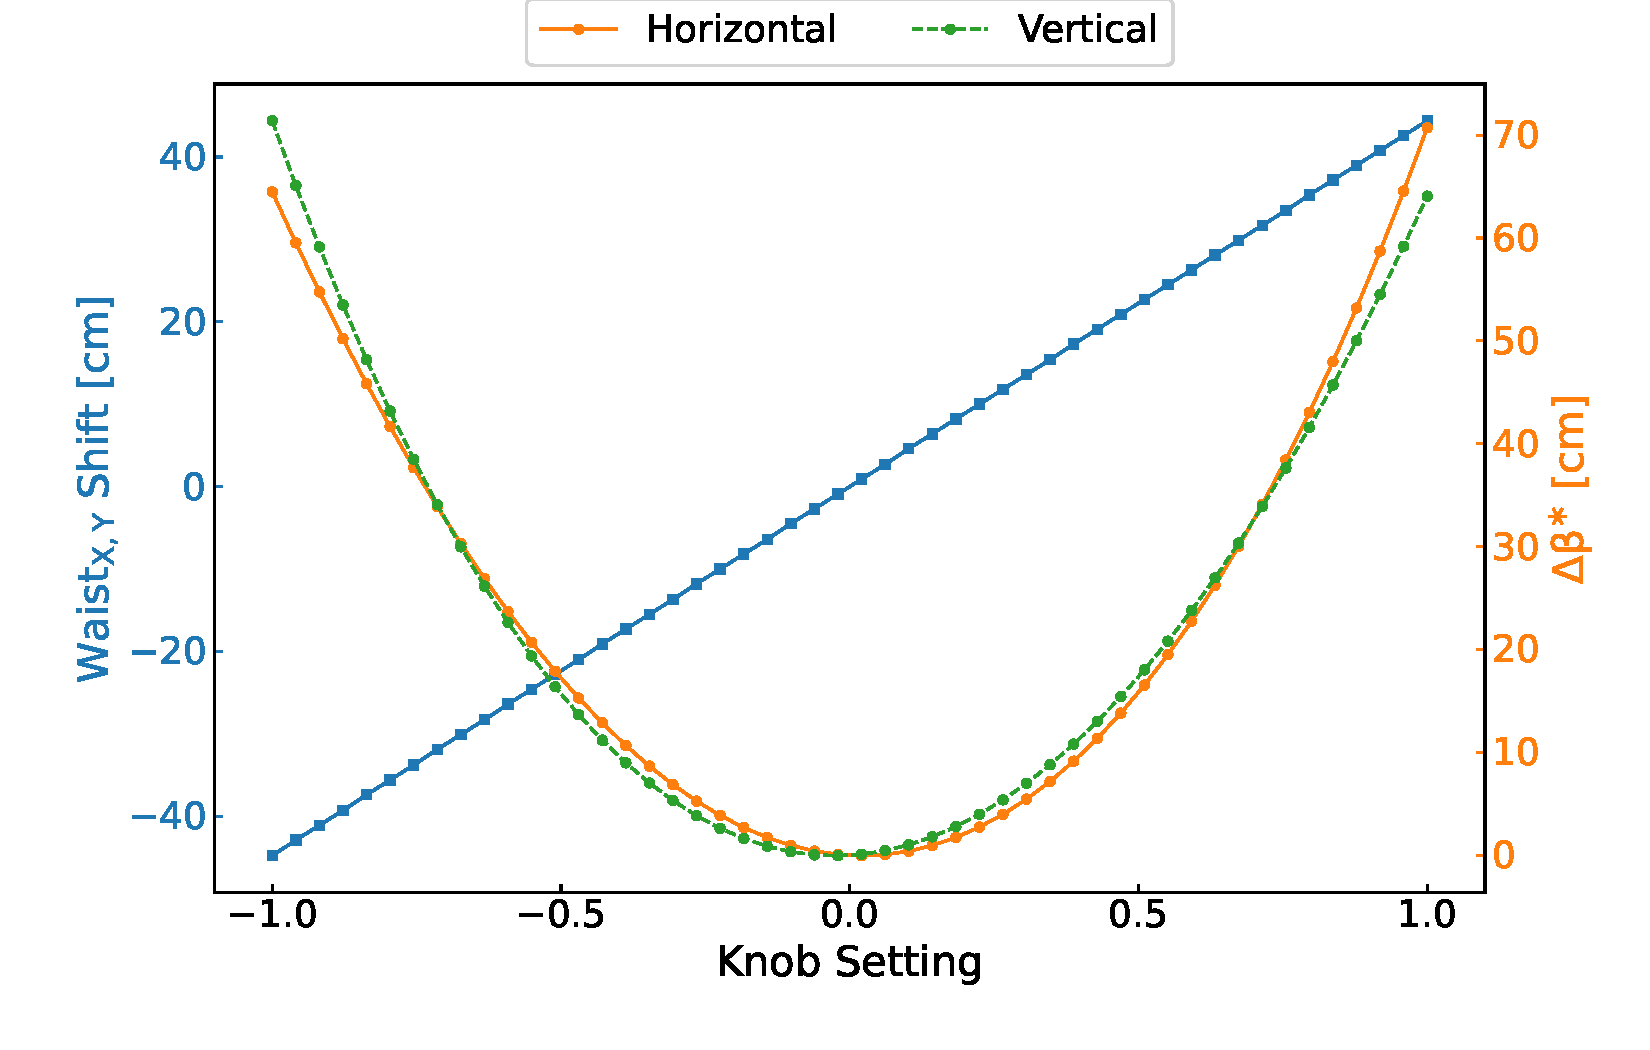
\includegraphics[width=\textwidth]{Figures/IR_Coupling_Correction/rigid_waist_shift_waist_effect_combined.pdf}
    \caption{Simulated effect of the designed Rigid Waist Shift knob as defined in \cref{table:rigid_waist_shift_knob} on the \(\beta^{\ast} =\)~\qty{30}{\centi\metre} optics of \num{2022}. The \textcolor{mplblue}{blue} line represents the waist displacement from the design location. The \textcolor{mplorange}{orange} and \textcolor{mplgreen}{green} lines represent the horizontal and vertical \(\beta\)-functions change at the IP as the waist is displaced, respectively.}
    \label{figure:rigid_waist_shift_knob_effect_on_waist}
\end{figure}

The waist displacement from the design location (\textcolor{mplblue}{blue} line) is almost completely linear with the knob setting.
One can note that the minima of the parabolas indicating the change of \(\beta\)-functions at the IP (\textcolor{mplblue}{blue} and \textcolor{mplorange}{orange} curves) are not found at exactly the zero knob setting, which is because the LHC design optics include a very small waist at IP\num{1} and IP\num{5}.

In \cref{figure:rigid_waist_shift_knob_effect_on_betas} one can observe how the \(\beta\)-functions are affected by the application of an RWS, also simulated with the \(\beta^{\ast} =\)~\qty{30}{\centi\metre} optics of \num{2022}.
In this simulation the lattice was sliced to improve the resolution of the data points, which explains the smoother lines compared to, for instance, \cref{figure:lhc_ir5_zoomed}.
One can observe how the (anti-)symmetry of the optics in the IR is broken when applying the knob (full vs dashed lines): the horizontal (\textcolor{mplb}{blue}) and vertical (\textcolor{mplr}{red}) \(\beta\)-functions do not mirror each other anymore.
Inset zooms are included around the location of the MQSX magnets (\textcolor{mqsx_green}{green} vertical lines), showing how the horizontal and vertical \(\beta\)-functions are modified in their vicinity.
The purpose of this setup is detailed in \cref{subsection:rws_application_and_simulations}.

\begin{figure}[!htb]
    \centering
    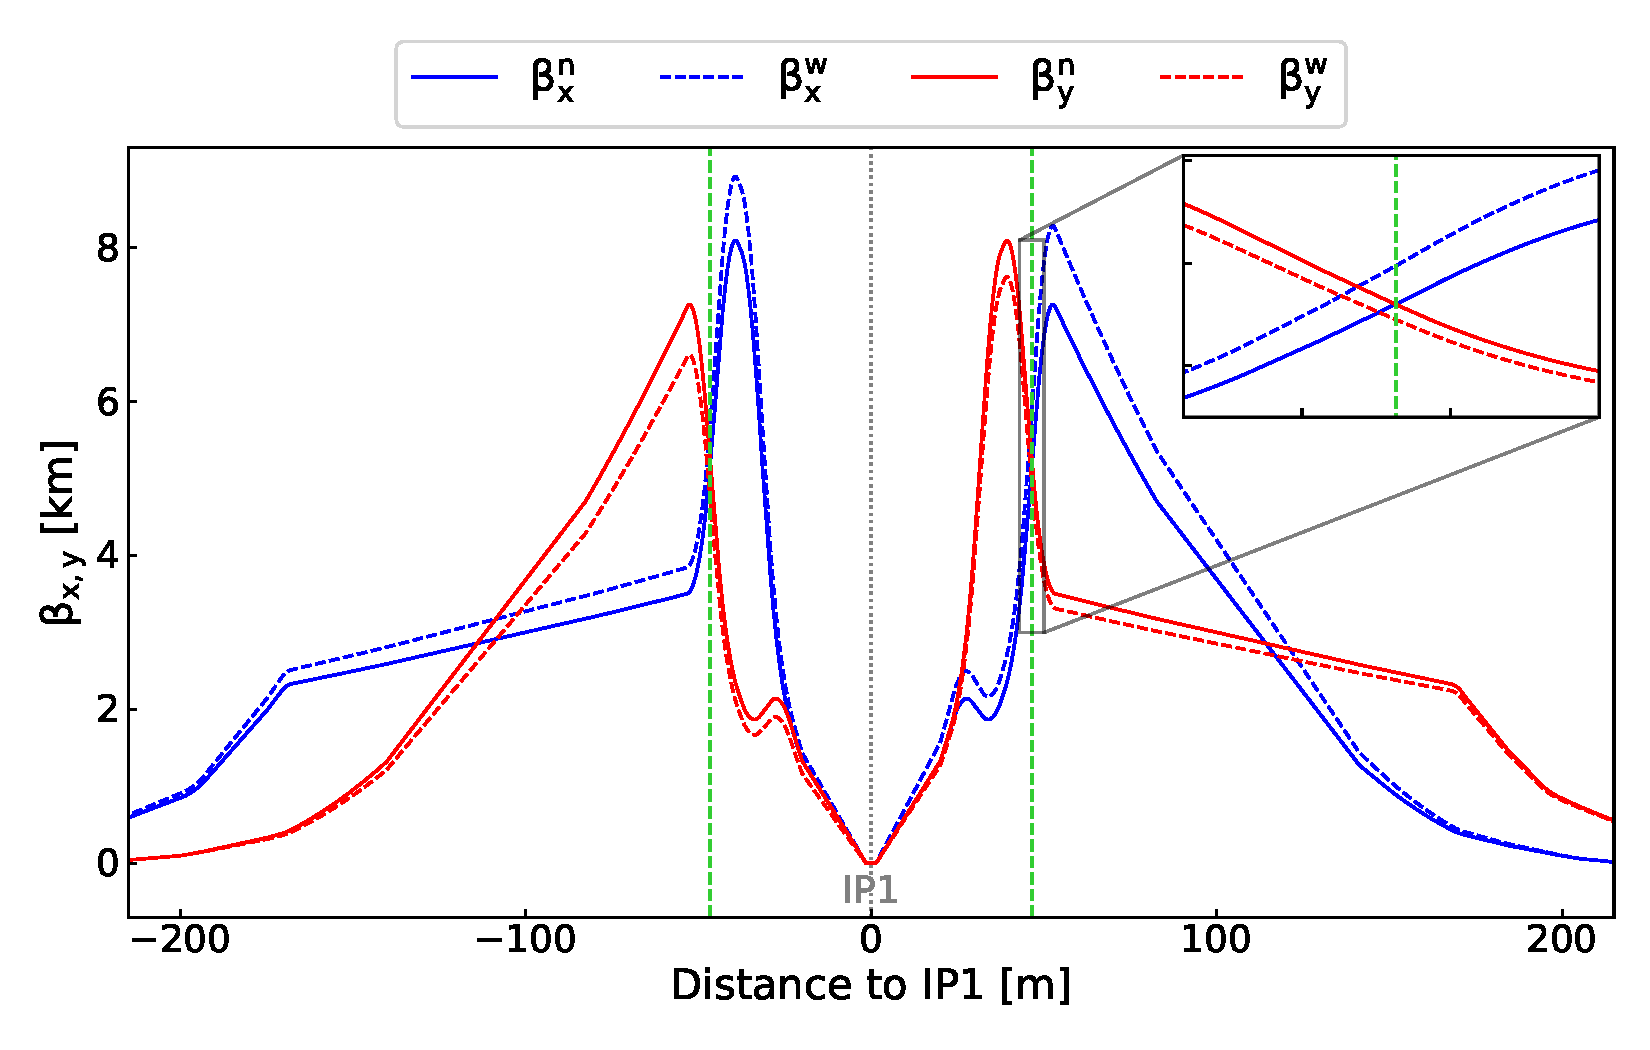
\includegraphics[width=\textwidth]{Figures/IR_Coupling_Correction/rigid_waist_shift_betas_effect.pdf}
    \caption{Simulated effect of the designed RWS knob on the \(\beta\)-functions around IP\num{1}, with the \(\beta^{\ast} =\)~\qty{30}{\centi\metre} optics of \num{2022}. The \(\beta\)-functions for both the horizontal (\textcolor{mplb}{blue}) and vertical (\textcolor{mplr}{red}) planes are shown for the nominal (full lines) and shifted waists (dashed lines) scenarios. An identical result is found for IP\num{5}.}
    \label{figure:rigid_waist_shift_knob_effect_on_betas}
\end{figure}

\subsubsection*{Optics Impact and Rematching}

Predictably, the application of a Rigid Waist Shift as described above has a strong impact on the optics across the machine.
This is due to the significant change of \(\beta\)-functions in the triplets, which sends a beating wave from the IR to the rest of the machine.
Applying an RWS with a unit setting of \num{1}, as defined in \cref{table:rigid_waist_shift_knob}, leads to a \numrange[range-phrase = --]{20}{30}\unit{\percent} increase in peak \gls{beta-beating} throughout the machine, depending on the observed beam and plane.

This can be observed in \cref{figure:rigid_waist_shift_betabeating}, where in simulations an RWS was implemented with a unit setting of \num{1} at IP\num{1} and the optics deviations from the nominal scenario were determined across the machine for both beams.
The most affected beam and plane depends on the setting of the RWS: in \cref{figure:rigid_waist_shift_betabeating} beam~\num{1} horizontal and beam~\num{2} vertical are most affected, but these would be beam~\num{1} vertical and beam~\num{2} horizontal if the RWS was applied with a setting of \num{-1}.
Naturally, some strong outliers can be observed in the vicinity of the IP, which correspond to the desired deviation at the IP and in the triplets induced by the \gls{knob} \gls{trim}.
\break

\begin{figure}[!htb]
    \centering
    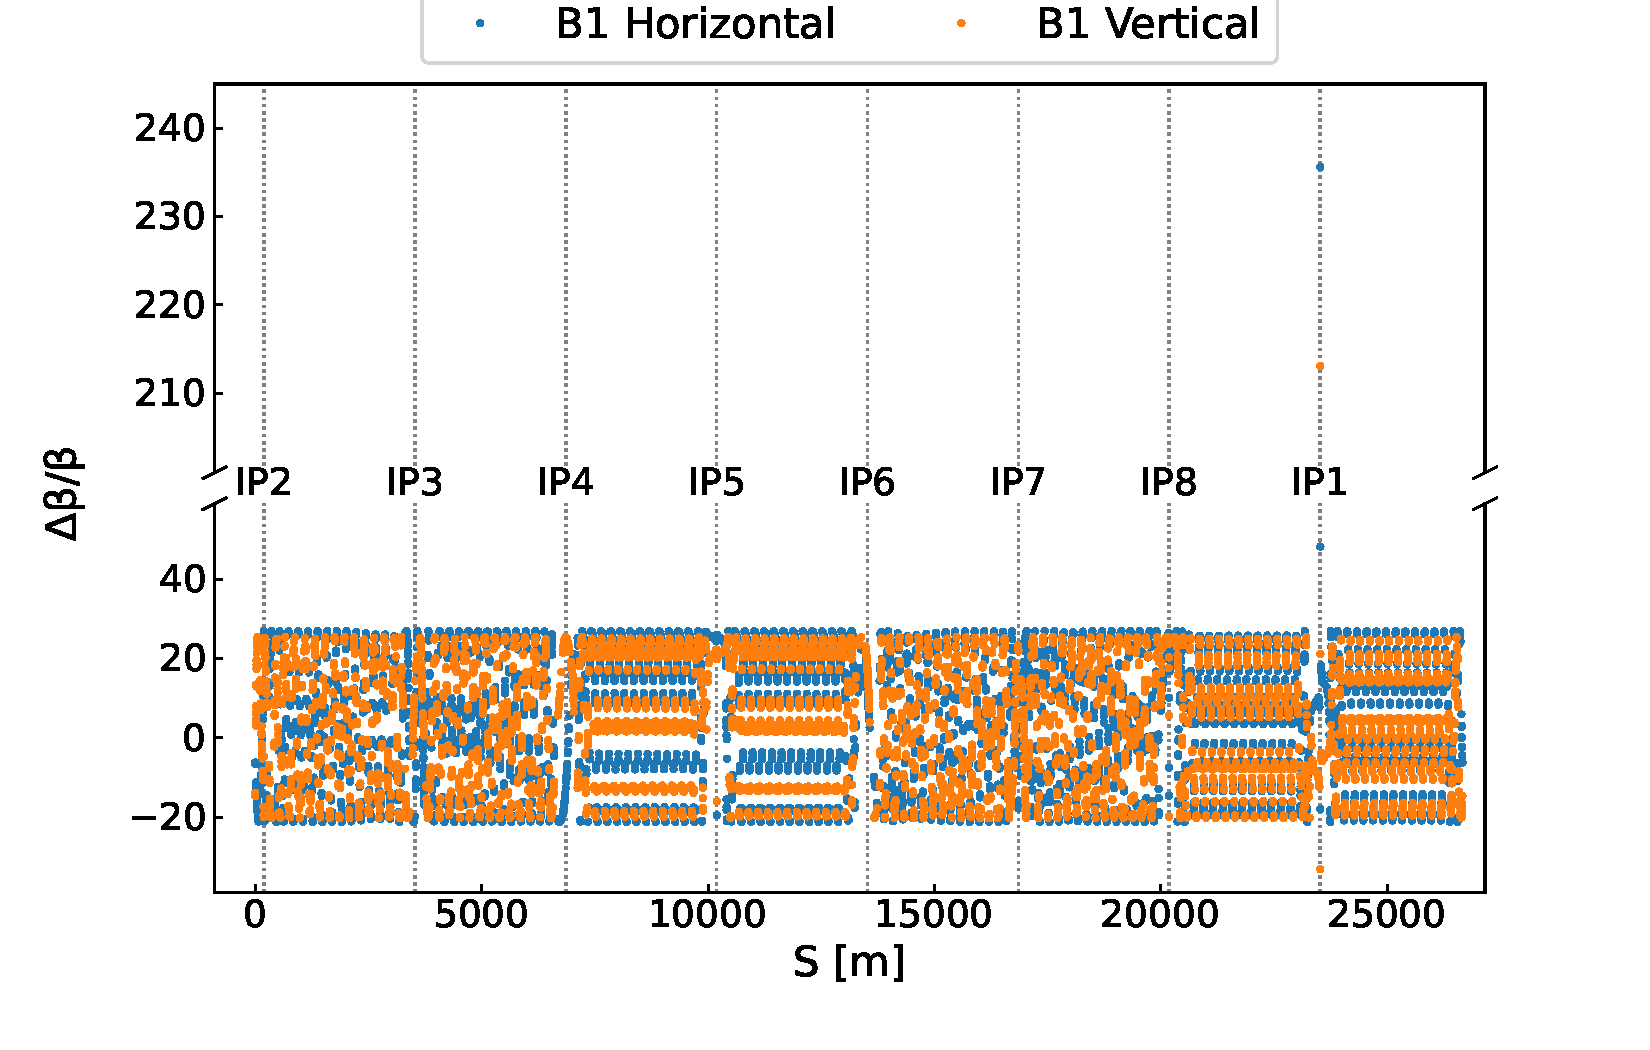
\includegraphics[width=\textwidth]{Figures/IR_Coupling_Correction/rws_ir1_b1_bbeating.pdf}
    \caption{Simulated \(\beta\)-beating induced across beam~\num{1} in both the horizontal (\textcolor{mplblue}{blue}) and vertical (\textcolor{mplorange}{orange}) planes, from applying an RWS as defined in \cref{table:rigid_waist_shift_knob} at IP\num{1}. A \numrange{20}{30}\unit{\percent} \(\beta\)-beating is observed through most of the machine, with (wanted) outliers close to IP\num{1}.}
    \label{figure:rigid_waist_shift_betabeating}
\end{figure}

Such a deviation of the optics has an impact on correction knobs.
For instance, simulations show that application of the RWS causes a \qty{15}{\percent} deviation from the achieved \glssymbol{Cminus} to the target value set through the LHC global coupling knobs, used for coupling correction with the arc skew quadrupoles.
Additionally, the optics deviations will change the impact of any errors probed while the RWS is trimmed in, namely the skew quadrupolar impact on the \gls{Cminus} (see \cref{equation:deltaqmin_guignard}).

In order to limit this impact on the optics and guarantee good measurements under an RWS, new correction knobs have been developed that make use of individually powered quadrupoles Q\num{4} to Q\num{10} (included). 
These knobs tune the optics functions and rematch them at the edges of the IR in the large sense.
They were designed with the \gls{MADX} code and a software developed for the occasion that can create these experimental configurations for a given IP in the machine~\cite{CODE:Soubelet:pyrws}.

These knobs are obtained from simulations after applying an RWS in a given IR and iterating several matching routines for quantities of interest at different locations in the machine.
Importantly, no involved magnet sees its powering change by more than \(\sim\)\qty{3}{\percent} with the application of these knobs, which allows for respecting the powering limits of individually powered elements.
As the rematching knobs depend on the RWS setting and optics configuration, many variations are possible and no general definition table is available akin to \cref{table:colinearity_knob,table:rigid_waist_shift_knob}.
A full definition of the rematching knobs for the \(\beta^{\ast} =\)~\qty{30}{\centi\meter} optics of 2022 as used in the LHC can be found in \cref{section:optics_rematching_knobs_lsa}.

\Cref{figure:rws_rematching_efficiency} shows a comparison of the simulated optics deviation in the beam~\num{1} horizontal plane, induced by the RWS before (\textcolor{mplblue}{blue}) and after (\textcolor{mplorange}{orange}) applying the rematching knob, here implemented at IP\num{1}.
Across the machine the \gls{beta-beating} is brought down by \(\sim\)\qty{20}{\percent} to around \(\sim\)\qty{5}{\percent} depending on the beam and plane compared to the nominal scenario, except for the vicinity of the IP where the desired deviation is kept unchanged.
A \qty{5}{\percent} \(\beta\)-beating across the machine is an acceptable level as it is similar to the level of control achieved during normal operation with all corrections trimmed in (see \cite{PRAB:Persson:LHC_Optics_Commissioning_OnePercent,CERN:Persson:LHCOpticsCorrectionsEvian2019}), as can be seen in \cref{figure:virgin_vs_corrected_lhcb2}.

While only beam~\num{1} horizontal is shown in this figure, results are similar for all planes of beam~\num{1} and beam~\num{2}.
As the rematching depends on the desired configuration (given optics and setting of the RWS) a knob has to be designed for each beam, at each IR and for each RWS setting.

\begin{figure}[!htb]
    \centering
    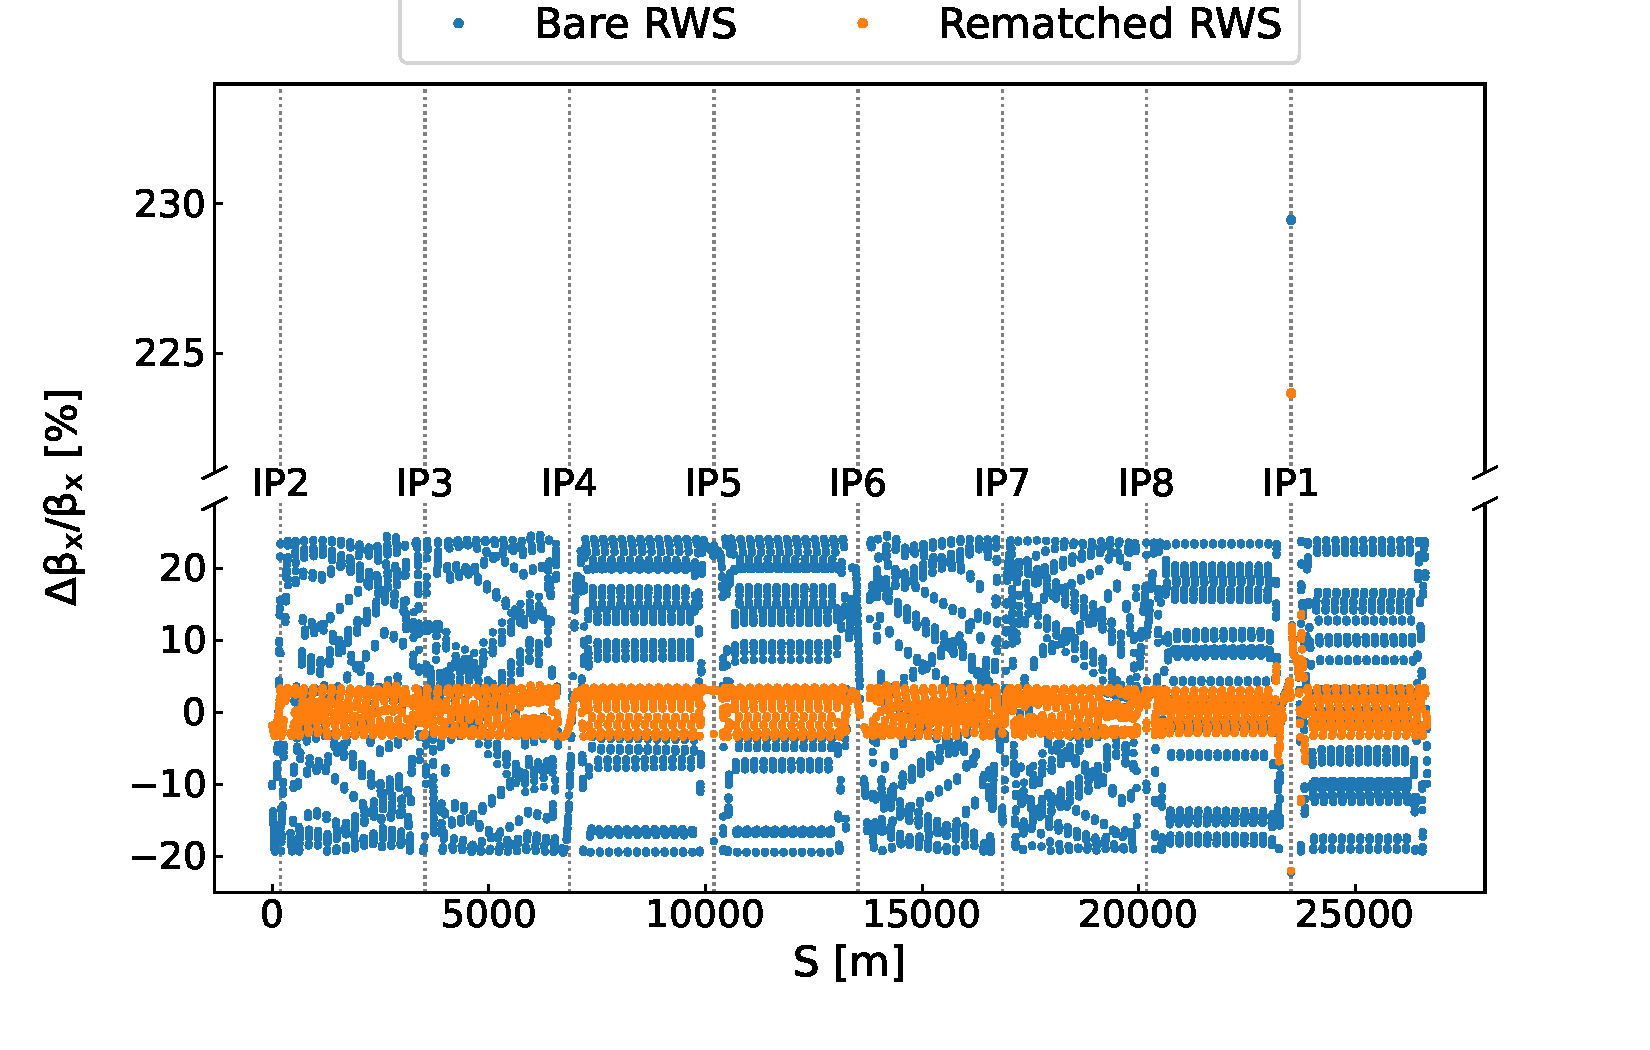
\includegraphics[width=\textwidth]{Figures/IR_Coupling_Correction/rws_ir1_b1_bbeating_rematched.pdf}
    \caption{Simulated \(\beta\)-beating induced across the machine in the beam~\num{1} horizontal plane from applying an RWS at IP\num{1}, before (\textcolor{mplblue}{blue}) and after (\textcolor{mplorange}{orange}) applying the optics rematching knob.}
    \label{figure:rws_rematching_efficiency}
\end{figure}

One can notice that near the IP the beating is also lowered by the rematching, but stays high enough to still break the symmetry of the IR.
\Cref{figure:rws_ir1_rematching_betas} shows the \(\beta\)-functions around IP\num{1} before (full lines) and after (dashed lines) application of the rematching knobs.
One can observe how the deviation between the two cases is negligible close to the IP and, importantly, in both cases the symmetry of the IR is broken compared to, for instance, \cref{figure:lhc_ir5_zoomed}.

\begin{figure}[!htb]
    \centering
    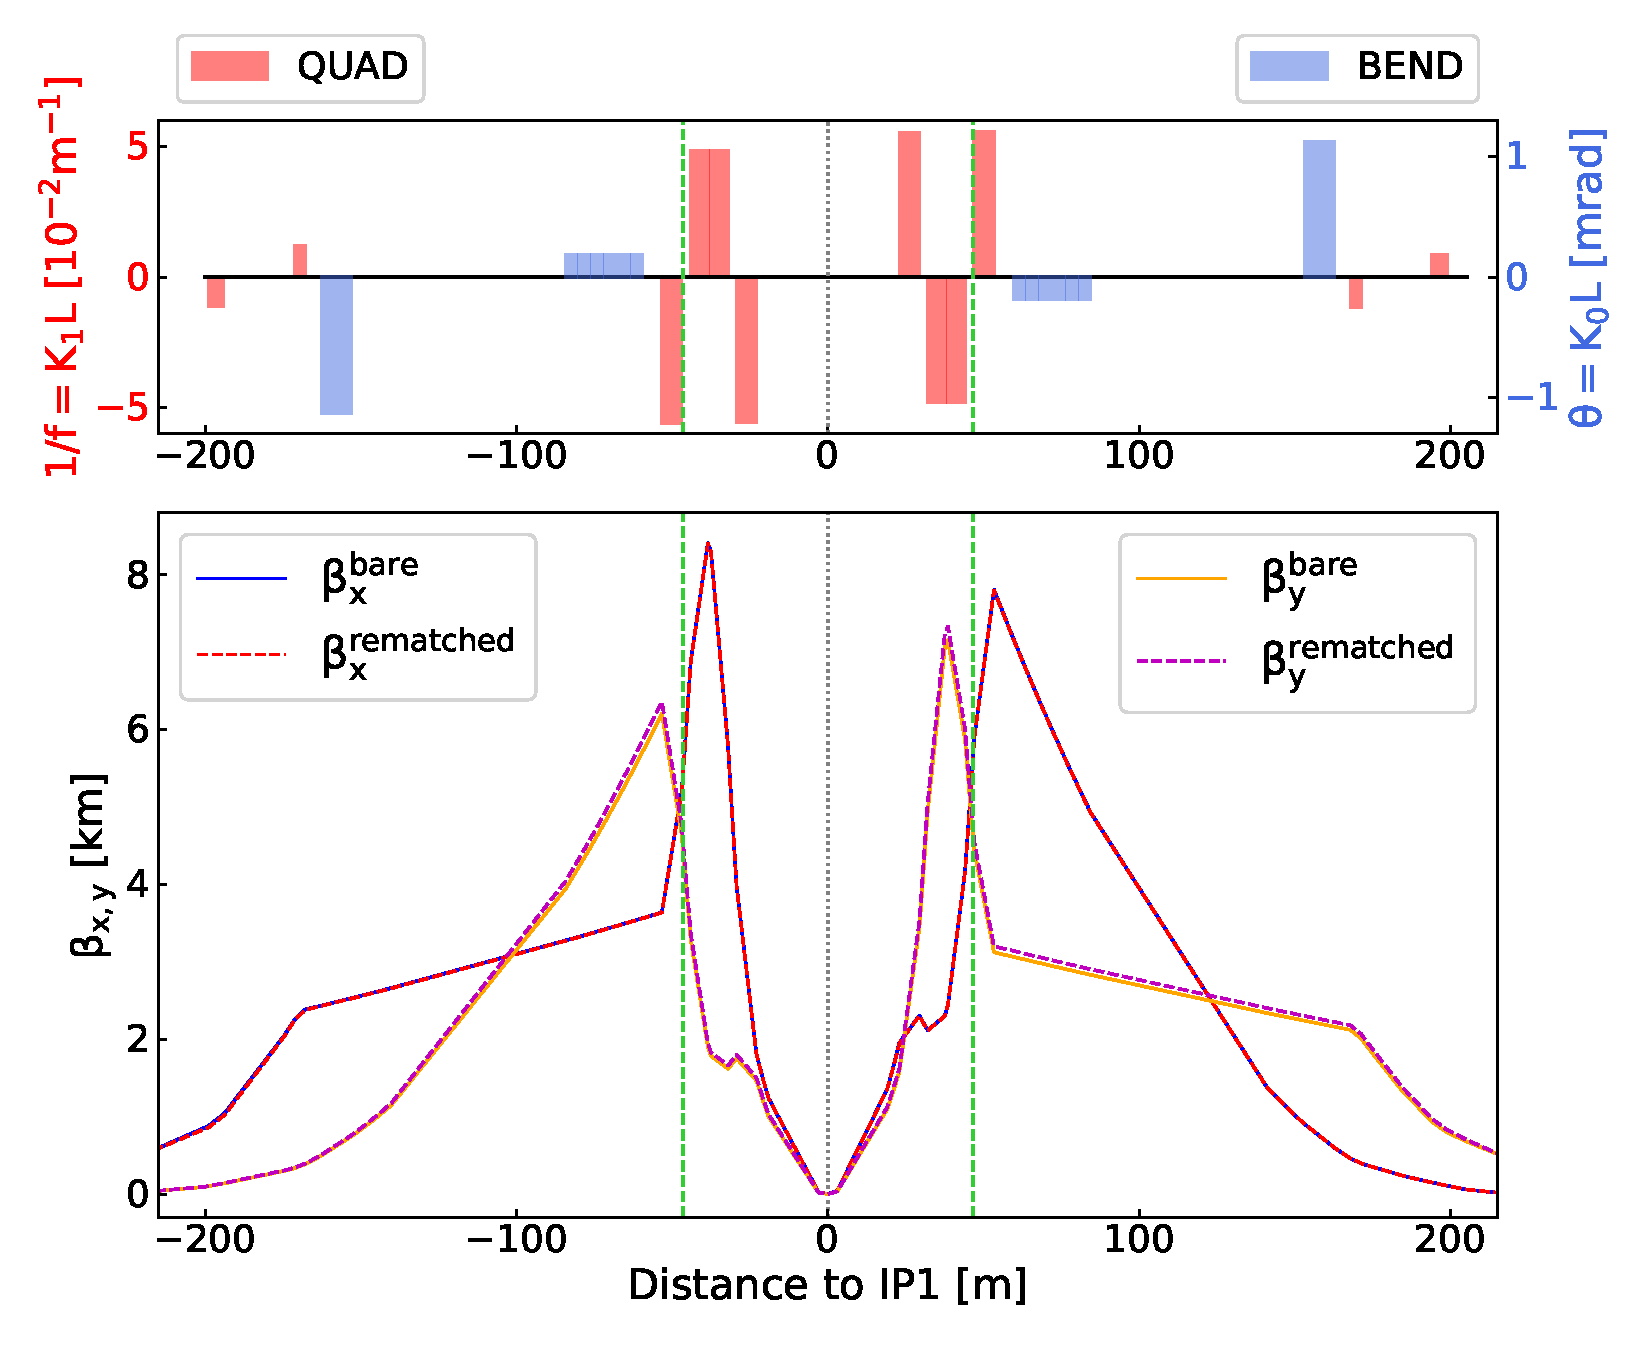
\includegraphics[width=\textwidth]{Figures/IR_Coupling_Correction/rws_ir1_rematching.pdf}
    \caption{Simulated \(\beta\)-functions around IP\num{1} when applying an RWS, before (full lines) and after (dashed lines) application of the rematching knobs, with the \(\beta^{\ast} =\)~\qty{30}{\centi\metre} optics of \num{2022}.}
    \label{figure:rws_ir1_rematching_betas}
\end{figure}

\subsection{Application Concept and Simulations}
\label{subsection:rws_application_and_simulations}

Making away with the optics symmetry of the \gls{IR} allows to break the locality of any coupling bump, even a truly local one.
As can be seen on the inset zooms of \cref{figure:rigid_waist_shift_knob_effect_on_betas}, with the application of an RWS the \(\beta\)-functions at the MQSX magnets change enough that the \(\sqrt{\beta_x \beta_y}\) term in \cref{equation:deltaqmin_only_mqsxs} are different at the two magnets.
\Cref{table:sqrt_betas_from_rws} shows the values of these terms with and without an RWS applied.
Phase advances are also changed, but by a very small amount.

\begin{table}[!htb]
    \centering
    \begin{tblr}{colspec={ccc}}
        \hline
        \SetCell[r=2,c=1]{m,c} \textbf{Magnet} & \SetCell[c=2]{c} \textbf{\(\sqrt{\beta_x \beta_y}\) [\unit{\square\meter}]}   \\
        \cline{2,3}                            &  Without an RWS            &    With an RWS                                   \\
        \hline
        MQSX.3L[IP]                            &    \num{5193.084265}       &     \num{5186.603944}                            \\
        MQSX.3R[IP]                            &    \num{5199.142377}       &     \num{5396.527580}                            \\
        \hline
    \end{tblr}
    \caption{Values of the \(\sqrt{\beta_x \beta_y}\) term in \cref{equation:deltaqmin_only_mqsxs} at the MQSX magnets around IP\num{1} or IP\num{5} without (left) and with (right) the application of an RWS, with the \(\beta^{\ast} =\)~\qty{30}{\centi\metre} optics of \num{2022}.}
    \label{table:sqrt_betas_from_rws}
\end{table}

\Cref{figure:rdt_leak} shows the coupling \glspl{RDT} from a closed coupling bump around the IP created through the colinearity knob, both in the presence (\textcolor{mplr}{red}) and absence (\textcolor{mplb}{blue}) of an RWS.

\begin{figure}[!htb]
    \centering
    \includegraphics*[width=\textwidth]{Figures/IR_Coupling_Correction/waist_shift_leaks_rdts.pdf}
    \caption{Amplitudes of the linear coupling RDTs in the vicinity of IP\num{1} under a coupling bump, with (\textcolor{mplr}{red}) and without (\textcolor{mplb}{blue}) an RWS. The vertical \textcolor{mqsx_green}{green} lines represent the positions of the skew quadrupoles correctors (MQSX.\num{3}[RL]\num{1}) used to implement the coupling bump. A colinearity knob setting of \num{10} and a rigidity waist shift knob setting of \num{1} were used.}
    \label{figure:rdt_leak}
\end{figure}
\break

When applying a Rigid Waist Shift and breaking the optics symmetry of the IR, one can observe a leakage of the coupling \glspl{RDT} outside the limits of the initial coupling bump.
These RDTs will then have a residual presence in the machine, which can be measured and reconstructed from turn-by-turn data from \glspl{BPM} with more suitable phase advances.
As a consequence, under an RWS even a local coupling bump that would normally be invisible to the rest of the machine will have a direct impact on the global coupling, measured as the \glssymbol{Cminus}.
This can be seen in \cref{figure:knob_to_cminus_with_waist}, where changes in the setting of the colinearity knob now have a strong effect on the \glssymbol{Cminus} when an RWS is applied in the relevant \gls{IR}.

\begin{figure}[!htb]
    \centering
    \includegraphics*[width=0.99\textwidth]{Figures/IR_Coupling_Correction/colin_knob_vs_waist_shift.pdf}
    \caption{Impact of the colinearity knob on the global \(\abs{C^{-}}\), calculated according to \cref{equation:deltaqmin_from_f1001}, with (\textcolor{mplblue}{blue}) and without (\textcolor{mplorange}{orange}) applying an RWS.}
    \label{figure:knob_to_cminus_with_waist}
\end{figure}

As previously mentioned, since the bump is not actually perfectly closed the \textcolor{mplorange}{orange} line in \cref{figure:knob_to_cminus_with_waist} is not completely flat and reaches up to \(\sim\)~\num{1e-5}, which is well below the measurement accuracy for the \(\abs{C^{-}}\).
The behavior seen in \cref{figure:knob_to_cminus_with_waist}, though theoretical, has been experimentally tested and confirmed in the machine~\cite{CERN:Persson:Local_Coupling_IP}.
Importantly, this behavior opens the possibility of using an RWS to probe IR local coupling through the measured global coupling.

Simulations have been done to investigate the feasibility of finding local coupling correction settings using an RWS, with the \(\beta^{\ast} = \) \qty{30}{cm} optics of \num{2022}.
At both IR\num{1} and IR\num{5} a local coupling bump was created by introducing identical tilt errors in triplet quadrupoles Q\num{3} - thus giving a skew quadrupolar component - and the colinearity knob was powered for compensation.
A full parameter space was explored, both with and without an RWS applied.
\Cref{figure:cminus_colin_vs_tilt_with_waist} shows the values of the resulting \(\abs{C^{-}}\) across the parameter space when an RWS is applied.
\Cref{figure:beam_size_colin_vs_tilt_no_waist} shows the resulting IP beam size increase as a ratio to the nominal beam size across the same parameter space.

\begin{figure}[!htb]
    \centering
    \includegraphics*[width=0.95\textwidth]{Figures/IR_Coupling_Correction/cminus_colin_tilt_compensation_with_waist.pdf}
    \caption{Resulting \(\abs{C^{-}}\) (\cref{equation:deltaqmin_from_f1001}) for various combinations of tilt error and colinearity knob settings, when applying an RWS.}
    \label{figure:cminus_colin_vs_tilt_with_waist}
\end{figure}

\begin{figure}[!htb]
    \centering
    \includegraphics*[width=0.95\textwidth]{Figures/IR_Coupling_Correction/ip_beam_size_growth_colin_tilt_compensation_no_waist.pdf}
    \caption{Resulting beam size (\cref{equation:lebedev_beam_size}) increase for identical settings of tilt error and colinearity knob settings as \cref{figure:cminus_colin_vs_tilt_with_waist}, but without an RWS.}
    \label{figure:beam_size_colin_vs_tilt_no_waist}
\end{figure}

The results of \cref{figure:beam_size_colin_vs_tilt_no_waist} highlight that minimization of the growth is possible, though a wrong setting would enhance the phenomenon.
A great correlation between beam size growth from the local coupling bump (without RWS, see \cref{figure:cminus_colin_vs_tilt_with_waist}) and the \glssymbol{Cminus} from leaked RDTs (with RWS, see \cref{figure:beam_size_colin_vs_tilt_no_waist}) is observed.

Simulations replicating a more complex scenario - akin to operational conditions - were also performed.
In these, tilt errors were introduced in triplet quadrupoles Q\num{3} as previously to create a closed local coupling bump around the IP.
Additionally, some tilt errors were added to an individually powered quadrupole in IR\num{5} (for instance Q\num{5}) to include the presence of expected residual local coupling errors in the other main IR, which contribute to the global coupling by the amount of \num{1e-3}.
Some global coupling sources were also added with a dedicated knob~\cite{CERN:Tomas:Optimizing_Global_Coupling_Knobs_LHC} that bring the global coupling to \num{1e-2}, which was then corrected through a routine and brought down to \(\sim\)\num{3e-3}, a level similar to what can be achieved in the machine~\cite{PRES:Persson:Transverse_Coupling_OMC_OP,PRES:Persson:Transverse_Coupling_Stability_HLLHC_WP2}.
The RWS and colinearity knobs were then powered to different settings, and the resulting \glssymbol{Cminus} and IP beam sizes were determined in all settings combinations.

Similar to the previous studies made for \cref{figure:cminus_colin_vs_tilt_with_waist,figure:beam_size_colin_vs_tilt_no_waist}, an entire parameter space of implemented errors and corrections has been explored.
The evolution of both the \(\abs{C^{-}}\) and the beam size growth at IP\num{1} for one of these simulations can be seen in \cref{figure:full_scenario_colin_correction_dqmin_lebedev}.
These curves would correspond to a vertical line in \cref{figure:cminus_colin_vs_tilt_with_waist,figure:beam_size_colin_vs_tilt_no_waist}, but with a realistic scenario.

\begin{figure}[!htb]
    \centering
    \includegraphics*[width=\textwidth]{Figures/IR_Coupling_Correction/full_scenario_cminus_and_ip_size.pdf}
    \caption{Resulting \(\abs{C^{-}}\) under an RWS (\textcolor{mplorange}{orange}) and IP\num{1} beam size (\cref{equation:lebedev_beam_size}) without an RWS relative to the nominal scenario (\textcolor{mplblue}{blue}), for various colinearity knob settings. The black dotted line represents the threshold of a \qty{1}{\percent} beam size increase from the nominal scenario.}
    \label{figure:full_scenario_colin_correction_dqmin_lebedev}
\end{figure}

It can be observed that settings minimizing the measured \(\abs{C^{-}}\) under an RWS are very close to minimizing the coupling induced beam size increase without said RWS.
Here these settings also compensate for the contribution of the other added sources, on top of the local ones.
Similarly to previous studies a great correlation is observed, and across the parameter space one computes a \num{0.96} Pearson correlation coefficient between the quantities shown in \cref{figure:full_scenario_colin_correction_dqmin_lebedev}.
This confirms the link between the measured \(\abs{C^{-}}\) and the quantities of interest at the IP location.
To summarize:

\begin{itemize}
    \item Thanks to the RWS, sources leading to truly local coupling can be probed through their forced impact on global coupling.
    \item Using the correlation properties demonstrated above, one can find settings to minimize said local coupling and its effects at the IP.
\end{itemize}

\subsection{Determining Corrections}

The corrections which would compensate only the local sources are determined by comparing the measured \(\abs{C^{-}}\) to simulations, such as the orange line in \cref{figure:full_scenario_colin_correction_dqmin_lebedev}.

In the real machine, some coupling will remain in the arcs due to a non-perfect global correction and non-local SbS corrections.
As the method probes local errors' impact through the \(\abs{C^{-}}\), it will naturally be sensitive to the global coupling in the machine, which should be replicated in simulations.
Although the overall behavior of simulations remains similar when including this component, an important change from the line seen in \cref{figure:full_scenario_colin_correction_dqmin_lebedev} is the location of the setting that minimizes the \(\abs{C^{-}}\).
The relevance of this property will be discussed below.
By comparing measurements from a colinearity knob scan to simulations - where the former includes the impact of local errors, but the latter does not - one can single out the contribution of the local sources to global coupling.
This is illustrated in \cref{figure:full_scenario_determine_correction}.

\begin{figure}[!htb]
    \centering
    \includegraphics*[width=0.95\textwidth]{Figures/IR_Coupling_Correction/full_scenario_determine_correction.pdf}
    \caption{Resulting \(\abs{C^{-}}\) in simulations as done for \cref{figure:full_scenario_colin_correction_dqmin_lebedev}, with (\textcolor{mplblue}{blue}) and without (\textcolor{mplorange}{orange}) local coupling sources in IR\num{1}.}
    \label{figure:full_scenario_determine_correction}
\end{figure}

\Cref{figure:full_scenario_determine_correction} shows the resulting \(\abs{C^{-}}\) values under an RWS during a colinearity knob scan, for one of the simulation scenarios mentioned previously (\cref{figure:full_scenario_colin_correction_dqmin_lebedev}) (\textcolor{mplblue}{blue}), and a similar scenario in which no local coupling sources were implemented in IR\num{1} (\textcolor{mplorange}{orange}).
The former represents what would be measured in the machine, including the contribution of local sources.
The latter represents a simulation to compare such a measurement to, which includes all contributions to global coupling except for the IR local sources.
The highlighted difference between the two curves is then fully explained by the local sources.

Applying a trim of the colinearity knob setting linearly translates the curves of \cref{figure:full_scenario_determine_correction} horizontally.
This behavior is valid and verifiable in both simulations and measurements.
Therefore, one looks to determine a colinearity knob trim that, if applied in the machine, would bring the measurement's \(\abs{C^{-}}\) minimization point to that of the simulation.
As this difference if fully explained by local sources, this trim contains the information on the local error in terms of colinearity knob setting: powering of the corrector magnets.
In \cref{figure:full_scenario_determine_correction} the minima are highlighted with vertical lines and the aforementioned correction trim is determined from the relative position of these two minima.
The value is different from that of the minimization in \cref{figure:full_scenario_colin_correction_dqmin_lebedev} as there global sources are also compensated while this correction aims at compensating only the local sources.

\begin{figure}[!htb]
    \centering
    \includegraphics*[width=0.95\textwidth]{Figures/IR_Coupling_Correction/full_scenario_correction_efficiency.pdf}
    \caption{Relative IP beam sizes when compared to the nominal scenario (\textcolor{mplblue}{blue}) when inputting the local errors used in the study for \cref{figure:full_scenario_determine_correction} (\textcolor{mplorange}{orange}) and after applying the suggested correction (\textcolor{mplgreen}{green}). The black dotted line represents the threshold of a \qty{1}{\percent} beam size increase from the nominal scenario.}
    \label{figure:full_scenario_correction_efficiency}
\end{figure}

When only considering the local sources used for the results in \cref{figure:full_scenario_determine_correction} and inputting the correction trim suggested, one obtains a good compensation of the beam sizes at IP\num{1}.
\Cref{figure:full_scenario_correction_efficiency} shows the impact of these local errors and the effect of applying the suggested correction trim.
The exactitude and effectiveness of the determined correction can be improved by performing more granular scans of the colinearity knob, but the values used are representative of what can be done in measurements.

\subsubsection*{Reproducing the Machine's Coupling}

The reproduction of the machine's global coupling in simulations becomes necessary as soon as strong non-IR sources are present, which is likely in the real machine.
Unfortunately the true distribution of sources in the machine is not known, and this reproduction can then be done in different ways.
In studies, various implementations were tested: random tilts in all quadrupoles, LHC specific knobs~\cite{CERN:Tomas:Optimizing_Global_Coupling_Knobs_LHC}, longitudinal misalignment of sextupoles, field errors in specific magnets or random combinations of the above.
The resulting \glssymbol{Cminus} for these can be seen in \cref{figure:global_coupling_modeling_impact}, where for each scenario the minimization point is highlighted by a vertical dashed line.

\begin{figure}[!hbt]
    \centering
    \includegraphics*[width=\textwidth]{Figures/IR_Coupling_Correction/global_sources_influence.pdf}
    \caption{Resulting simulated \(\abs{C^{-}}\) under an RWS during a scan of the colinearity knob, for various implementations of global coupling in the machine. For each case a vertical dashed line highlights the location of the minimization point.}
    \label{figure:global_coupling_modeling_impact}
\end{figure}

In all investigated scenarios the achieved \(\abs{C^{-}}\) before applying the RWS is the same value before (\(\sim 10^{-2}\)) and after (\(\sim 2 \cdot 10^{-3}\)) applying a correction routine.
It was found that, to the levels of coupling we achieve after correcting the machine the distribution and implementation of sources had little impact on the minimization point of the \(\abs{C^{-}}\) curve under an RWS, as long as the overall pattern of the \(f_{1001}\) and the level of coupling measured in the machine were accurately reproduced.

One can see in \cref{figure:global_coupling_modeling_impact} how the minimization point is relatively unchanged by the global coupling implementation method within the precision of the mesh step used for the scan, which was chosen to reflect that achievable in the machine.
As a consequence, in simulations this reproduction was done by including the coupling correction knobs implemented in the machine, as determined during earlier commissioning steps.

\subsection{Rigid Waist Shift Procedure}

To summarize so far, two tools have been developed and presented to tackle local coupling correction:
\begin{itemize}
    \item The colinearity knob (\cref{table:colinearity_knob}) allows adjusting the coupling at the \gls{IP} without affecting the rest of the machine, namely previously established corrections.
    \item The \acrlong{RWS} knob (\cref{table:rigid_waist_shift_knob}) allows probing local errors through the \glssymbol{Cminus} (\cref{figure:rdt_leak,figure:knob_to_cminus_with_waist}) and to find a correction setting of the colinearity knob that will minimize the coupling at the \gls{IP} (\cref{figure:full_scenario_determine_correction,figure:full_scenario_correction_efficiency}).
\end{itemize}

Using those, the complete correction procedure for local linear coupling is then made of three steps:
\begin{enumerate}
    \item Firstly, calculating and applying a correction of the IR contribution to global coupling based on RDTs from turn-by-turn measurements, using the SbS technique.
    \item Secondly, breaking the optics symmetry between the right and left-hand side of the IP by applying an RWS, and performing a scan of the colinearity knob.
    \item Finally, analyzing the measurements data and comparing it to simulations in order to find a colinearity knob adjustment setting that minimizes the global coupling, without impacting the correction found in step~\num{1}.
\end{enumerate}

These measurements can be performed for each IR and for each beam, and the subsequent determined corrections can then be directly applied in the machine.

\section{Local Coupling Correction in the LHC 2022 Commissioning}
\label{section:rws_experimental_results}

Below are presented experimental results of local coupling correction in the \acrshort{LHC}'s first year of \Gls{run}~\num{3}, during the \num{2022} commissioning, using the \gls{RWS} procedure presented above.
One can refer to \cref{appendix:measurement_fills} for information on the fills used for experimental measurements.

\subsection{Segment-by-Segment Corrections}
\label{subsection:sbs_corrections}

In October \num{2021} a week of beam tests was done in the LHC at injection energy.
From the measurements at \qty{450}{\giga\electronvolt} a first set of local coupling corrections were calculated for each of the four main \glspl{IR} using the segment-by-segment technique.
\Cref{figure:beam_test_sbs_abs_f1001_ip5} shows the segment-by-segment results for the absolute value of the \(f_{1001}\) \gls{RDT} in IR\num{5}, from the \num{12}\({}^\mathrm{th}\) BPM left to right of IP\num{5}.
The vertical grey line indicates the location of the IP in the segment.
Due to the \gls{skew} quadrupole correctors in the IRs being single aperture magnets, one needs to find a single powering setting that works for both beams and both are shown on the figure.

\begin{figure}[!htb]
    \centering
    \includegraphics*[width=\textwidth]{Figures/IR_Coupling_Correction/beamtest_sbs_abs_f1001_ip5.pdf}
    \caption{Propagation of the measured \(\abs{f_{1001}}\) (\textcolor{mplblue}{blue}) around IP\num{5} (dashed grey line) and of the reconstructed values from the determined correction (\textcolor{mplorange}{orange}), measured at \qty{450}{\giga\electronvolt} and \(\beta^{*}=\) \qty{11}{\meter}.}
    \label{figure:beam_test_sbs_abs_f1001_ip5}
\end{figure}

One can see that the determined correction in IR\num{5} matches the propagated measurement within the tolerance of the error bars at the edges of the segment.
This guarantees a good compensation of the IR's contribution to global coupling.

During the LHC Run~\num{3} commissioning, local coupling corrections determined during the previous year's beam test were trimmed in the machine from the start.
After reaching the \(\beta^{*}=\) \qty{30}{\centi\meter} optics, where the machine is more sensitive to local errors, a noticeable deviation around IP\num{1} was observed and a refinement of the correction was determined, still with the segment-by-segment technique.
\Cref{figure:commissioning_sbs_real_f1001_ip1,,figure:commissioning_sbs_imag_f1001_ip1} show the effect of the new correction on the real and imaginary parts of the \(f_{1001}\) RDT in the segment, respectively.

\begin{figure}[!htb]
    \centering
    \includegraphics*[width=\textwidth]{Figures/IR_Coupling_Correction/commissioning_sbs_real_f1001_ip1.pdf}
    \caption{Propagation of the measured \(\Re f_{1001}\) (\textcolor{mplblue}{blue}) around IP\num{1} (dashed grey line) and the reconstructed values from the determined correction (\textcolor{mplorange}{orange}), measured at \qty{6.8}{\tera\electronvolt} and \(\beta^{*}=\) \qty{30}{\centi\meter}.}
    \label{figure:commissioning_sbs_real_f1001_ip1}
\end{figure}
  
\begin{figure}[!htb]
    \centering
    \includegraphics*[width=\textwidth]{Figures/IR_Coupling_Correction/commissioning_sbs_imag_f1001_ip1.pdf}
    \caption{Propagation of the measured \(\Im f_{1001}\) (\textcolor{mplblue}{blue}) around IP\num{1} (dashed grey line) and the reconstructed values from the determined correction (\textcolor{mplorange}{orange}), measured at \qty{6.8}{\tera\electronvolt} and \(\beta^{*}=\) \qty{30}{\centi\meter}.}
    \label{figure:commissioning_sbs_imag_f1001_ip1}
\end{figure}

The beating observed from the old correction was re-matched thanks to a setting adjustment where the IR\num{1} right-hand side corrector's powering was changed by \qty{1e-4}{\per\square\meter}.
The final correction settings determined with the segment-by-segment technique and trimmed in the machine at the four main \glspl{IR} can be found in \cref{table:sbs_corrections}, along with their counterpart values from \Gls{run}~\num{2} for comparison.

% \begin{table}[!htb]
%     \centering
%     \begin{tblr}{colspec={ccc}}
%         \hline
%         \SetCell[r=2,c=1]{c} \textbf{Circuit} & \SetCell[c=2]{c} \textbf{\(K_{1\mathrm{S}}\)~[\qty{1e-4}{\per\square\meter}]}              \\
%         \cline{2,3}
%                                  &    \textbf{2016-2018}~\cite{CERN:Persson:LHCOpticsCorrectionsEvian2019}    &    \textbf{2022 SbS}  \\
%         \hline
%             \textbf{RQXS.3L1}    &    \num{11}                                                                &     \num{8}           \\
%             \textbf{RQXS.3R1}    &    \num{7}                                                                 &     \num{7}           \\
%             \hline[dashed]
%             \textbf{RQXS.3L2}    &    \num{-14}                                                               &     \num{-14}         \\
%             \textbf{RQXS.3R2}    &    \num{-14}                                                               &     \num{-14}         \\
%             \hline[dashed]
%             \textbf{RQXS.3L5}    &    \num{7}                                                                 &     \num{6}           \\
%             \textbf{RQXS.3R5}    &    \num{7}                                                                 &     \num{6}           \\
%             \hline[dashed]
%             \textbf{RQXS.3L8}    &    \num{-5}                                                                &     \num{-5}          \\
%             \textbf{RQXS.3R8}    &    \num{-5}                                                                &     \num{-5}          \\
%         \hline
%     \end{tblr}
%     \caption{Local IR skew quadrupole correctors powering at the four main LHC IRs as determined with the segment-by-segment technique in the \num{2022} commissioning (right) and their values as used during the LHC Run~\num{2} (left).}
%     \label{table:sbs_corrections}
% \end{table}

\begin{table}[!htb]
    \centering
    \begin{tblr}{colspec={cccc}}
        \hline
        \SetCell[r=2,c=1]{c} \textbf{IR}  &  \SetCell[r=2,c=1]{c} \textbf{Circuit} & \SetCell[c=2]{c} \textbf{\(K_{1\mathrm{S}}\)~[\qty{1e-4}{\per\square\meter}]}                    \\
        \cline{3,4}
                                          &                                        &  \textbf{2016-2018}~\cite{CERN:Persson:LHCOpticsCorrectionsEvian2019}    &    \textbf{2022 SbS}  \\
        \hline
        \SetCell[r=2,c=1]{c} \textbf{IR1} &  \textbf{RQXS.3L1}                     &  \num{11}                                                                &     \num{8}           \\
                                          &  \textbf{RQXS.3R1}                     &  \num{7}                                                                 &     \num{7}           \\
        \hline[dashed]
        \SetCell[r=2,c=1]{c} \textbf{IR2} &  \textbf{RQXS.3L2}                     &  \num{-14}                                                               &     \num{-14}         \\
                                          &  \textbf{RQXS.3R2}                     &  \num{-14}                                                               &     \num{-14}         \\
        \hline[dashed]
        \SetCell[r=2,c=1]{c} \textbf{IR5} &  \textbf{RQXS.3L5}                     &  \num{7}                                                                 &     \num{6}           \\
                                          &  \textbf{RQXS.3R5}                     &  \num{7}                                                                 &     \num{6}           \\
        \hline[dashed]
        \SetCell[r=2,c=1]{c} \textbf{IR8} &  \textbf{RQXS.3L8}                     &  \num{-5}                                                                &     \num{-5}          \\
                                          &  \textbf{RQXS.3R8}                     &  \num{-5}                                                                &     \num{-5}          \\
        \hline
    \end{tblr}
    \caption{Local IR skew quadrupole correctors powering at the four main LHC IRs as determined with the segment-by-segment technique in the \num{2022} commissioning and their values as used during the LHC Run~\num{2}.}
    \label{table:sbs_corrections}
\end{table}

\subsection{Rigid Waist Shift Corrections}
\label{subsection:rws_pos_measurements_corrections}

The RWS method was implemented in both IR\num{1} and IR\num{5} at \qty{6.8}{\tera\electronvolt} and \(\beta^{*}=\) \qty{30}{\centi\meter} to determine final correction settings in the form of adjustments from the SbS corrections presented above.
Relevant fills used for these measurements can be found in \cref{table:run3_fills}.
\break

As a first step, the validity of the experimental setup was verified by trimming the RWS in the machine and then checking the efficiency of the optics rematching knobs.
\Cref{figure:ir5_rws_rematching} shows the \gls{beta-beating} across the machine for beam~\num{1} before any knob application (\textcolor{butter}{yellow}), from applying the RWS in IR\num{5} (\textcolor{skyblue}{blue}) and after the application of the optics re-matching knob (\textcolor{scarletred}{red}).
Similar checks were done for both beams and both IRs.
The \glspl{beta-function} in these measurements are reconstructed with the \acrshort{OMC} codes according to~\cite{PRAB:Wegscheider:Analytical_N_BPM}.

The measured impact is in agreement with what was expected from earlier simulations (see \cref{subsection:rigid_waist_shift}), leading to a \num{15}-\qty{25}{\percent} additional \(\beta\)-beating in the machine depending on the observed beam and plane; while the re-matching knob brought this beating back to about \qty{5}{\percent} where it was previously kept thanks to existing corrections.
Considering the state of the machine at the time of these measurements, it can be considered that the optics re-matching shows great efficiency.
Naturally, some strong deviations are noticed close to IP\num{5} (going out of range of the y-axis) as the optics there are changed on purpose, but also because \(\beta\)-functions reconstruction close the IPs is of relatively low quality.

After confirming the validity of the optics knobs and with the waist shift in the machine, scans of the colinearity knob (\cref{table:colinearity_knob}) were performed.
At each setting, a few measurements were taken by method of beam excitation, from which the coupling \glspl{RDT} were computed.
As the \gls{optics} are affected - and re-matched - differently for beam~\num{1} and beam~\num{2}, a scan of the colinearity knob was performed for each beam and for each IR.
Different scans were done with different granularity due to time constraints.

\begin{figure}[!htb]
    \centering
    \includegraphics*[width=\textwidth]{Figures/IR_Coupling_Correction/rematching_knob_efficiency.pdf}
    \caption{The beam~\num{1} \(\beta\)-beating observed at \qty{6.8}{\tera\electronvolt} and \(\beta^{*}=\)~\qty{30}{\centi\meter} for the corrected machine (\textcolor{butter}{yellow}), from the implementation of the RWS in IR\num{5} (\textcolor{skyblue}{blue}) and after applying the optics re-matching knob (\textcolor{scarletred}{red}). The highlighted area (\textcolor{highlightorange}{orange}) shows where magnetic elements are affected by the knobs.}
    \label{figure:ir5_rws_rematching}
\end{figure}

For each measurement the RDTs across the machine are normalized to the base case with no RWS, global coupling corrected and no colinearity knob trim.
Only then is the \glssymbol{Cminus} computed according to \cref{equation:deltaqmin_from_f1001}.
Then the variations due to the changes of the colinearity knob are visualized and compared to simulations.
In said simulations, the global coupling of the machine is reproduced by introducing the coupling correction knobs implemented in the machine at the time of measurements.

In \cref{figure:ir1_b1_pos_measurement,figure:ir1_b2_pos_measurement,figure:ir5_b1_pos_measurement,figure:ir5_b2_pos_measurement} comparisons are shown between simulations and scan measurements at IR\num{1} for beam~\num{1} and beam~\num{2}, then IR\num{5} for beam~\num{1} and beam~\num{2}, respectively.
The delta between minimization settings, corresponding to the suggested correction adjustment, is highlighted on each plot.
The relatively low range of achieved \glssymbol{Cminus} values is due to the aforementioned \glspl{RDT} normalization.
The noticeably different behavior of beam~\num{1} and beam~\num{2} simulations is explained by the different coupling situation in each beam: throughout commissioning beam~\num{2} has showcased little global coupling to be corrected while beam~\num{1} required significantly stronger global coupling corrections, as well as local adjustments for different arcs.
As these are reproduced in simulations, this difference in behavior is unsurprising.

\begin{figure}[!htb]
    \centering
    \includegraphics*[width=0.94\textwidth]{Figures/IR_Coupling_Correction/rws_measurement_ir1_b1_pos.pdf}
    \caption{Measurement scan done at IR\num{1} for beam \num{1} (\textcolor{mplr}{red}) and simulations for the same setup (\textcolor{mplblue}{blue}). The minima of both curves are highlighted by vertical dashed lines and the delta between the two, suggesting the remaining error to correct, is displayed on the graph.}
    \label{figure:ir1_b1_pos_measurement}
\end{figure}

\begin{figure}[!htb]
    \centering
    \includegraphics*[width=0.94\textwidth]{Figures/IR_Coupling_Correction/rws_measurement_ir1_b2_pos.pdf}
    \caption{Measurement scan done at IR\num{1} for beam \num{2} (\textcolor{mplr}{red}) and simulations for the same setup (\textcolor{mplblue}{blue}). The minima of both curves are highlighted by vertical dashed lines and the delta between the two, suggesting the remaining error to correct, is displayed on the graph.}
    \label{figure:ir1_b2_pos_measurement}
\end{figure}

\begin{figure}[!htb]
    \centering
    \includegraphics*[width=0.94\textwidth]{Figures/IR_Coupling_Correction/rws_measurement_ir5_b1_pos.pdf}
    \caption{Measurement scan done at IR\num{5} for beam \num{1} (\textcolor{mplr}{red}) and simulations for the same setup (\textcolor{mplblue}{blue}). The minima of both curves are highlighted by vertical dashed lines and the delta between the two, suggesting the remaining error to correct, is displayed on the graph.}
    \label{figure:ir5_b1_pos_measurement}
\end{figure}

\begin{figure}[!htb]
    \centering
    \includegraphics*[width=0.94\textwidth]{Figures/IR_Coupling_Correction/rws_measurement_ir5_b2_pos.pdf}
    \caption{Measurement scan done at IR\num{5} for beam \num{2} (\textcolor{mplr}{red}) and simulations for the same setup (\textcolor{mplblue}{blue}). The minima of both curves are highlighted by vertical dashed lines and the delta between the two, suggesting the remaining error to correct, is displayed on the graph.}
    \label{figure:ir5_b2_pos_measurement}
\end{figure}

In \cref{figure:ir1_b1_pos_measurement,figure:ir1_b2_pos_measurement,figure:ir5_b1_pos_measurement,figure:ir5_b2_pos_measurement}, simulations for beam~\num{2} suggest that the (small) reproduced global coupling has little effect on the procedure, and the colinearity knob scan could almost be used alone to determine the corrections.
For beam~\num{1} simulations however the impact of the reproduced global coupling appears much more substantial, as was the case in the machine, and this highlights the need to compare the scan measurements to simulations.
Overall, this comparison is needed in the case that there are significant coupling errors in the arcs.
It is worth noting that both beams' measurements converge to similar correction suggestions.
\break

\Cref{table:rws_corrections_summary} shows a summary of the suggested correction settings for each beam and IR.
While slightly different corrections are suggested from independent scans of beam~\num{1} and beam~\num{2}, it is possible that both values are simultaneously true.
Indeed, while most of the error contribution is expected to come from the dual-beam triplet quadrupoles and be common to both beams, errors in double aperture magnets Q\num{4} to Q\num{10} would affect each beam individually and force a divergence of the suggested correction adjustments for each beam.\\

\begin{table}[!htb]
    \centering
    $\begin{tblr}{colspec={ccc}}
        \hline
        \SetCell[r=2,c=1]{m,c} \textbf{Scan} & \SetCell[c=2]{c} \textbf{Suggested \( \Delta k \)~[\(10^{-4}\)\unit{\meter^{-2}}]} \\
        \cline{2,3}
                                             &  \textbf{Beam~\num{1}}  &  \textbf{Beam~\num{2}}     \\
        \hline
        \textbf{IR1}                         &  \num{-3.5}             &  \num{-3}                   \\
        \hline[dashed]
        \textbf{IR5}                         &  \num{-2}               &  \num{-1.5}                 \\
        \hline
    \end{tblr}$
    \caption{Correction adjustments suggested from the Rigid Waist Shift scans analysis, on top of the existing segment-by-segment corrections that were in the machine (see \cref{table:sbs_corrections}).}
    \label{table:rws_corrections_summary}
\end{table}

Furthermore, the orbit and hence feed-down but also the \(\beta\) ratio between sources and correctors are different for both beams, which could explain part of the difference.
As the main contributors to the error are the triplets, it is not unsurprising to obtain similar correction suggestions for both beams.

Some more measurements were performed with an opposite setting of the \gls{RWS} in both \glspl{IR} that did not yield sensible correction suggestions, which have not been shown here.
For completeness, these are exposed in \cref{appendix:inconclusive_measurements} together with the suspected reasons for each one's failure.

\subsection{Luminosity Confirmation}
\label{subsection:lumi_correction_trims}

Later on during the \num{2022} physics run, beam time was allocated to trim in the suggested adjustments from \cref{table:rws_corrections_summary}.
The impact of the corrections was assessed based on instantaneous luminosity measurements at the time of the trims.
Time was found to perform measurements of the efficiency of corrections in each IR at both \(\beta^{\ast} =\)~\qty{30}{\centi\meter} and \(\beta^{\ast} =\)~\qty{42}{\centi\meter}.
Information on the fills used can be found in \cref{table:md_fills}.

For each measurement, trims around the suggested correction adjustments were also performed in order to look for the best local setting, which might not necessarily have been found by the method.
Below are shown data from the trims at \(\beta^{\ast} =\)~\qty{30}{\centi\meter} only, while \(\beta^{\ast} =\)~\qty{42}{\centi\meter} results are compiled in a later table.

\Cref{figure:corrections_trims_ir1} shows the trim performed at IR\num{1} (\textcolor{mplblue}{blue}) and subsequent measured luminosity changes at the \acrshort{ATLAS} experiment (\textcolor{mplorange}{orange}).
The light blue area highlights the trim values suggested by the RWS method, which vary for beam~\num{1} and beam~\num{2}.
The instantaneous luminosity signal slightly trails up after the end of the correction adjustment trim as the ATLAS experiment publishes a time-averaged value.
A great improvement in luminosity can be observed from the trim, with an almost \qty{10}{\percent} improvement from the adjustment.

\begin{figure}[!htb]
    \centering
    \includegraphics*[width=\textwidth]{Figures/IR_Coupling_Correction/corrections_trim_ir1.pdf}
    \caption{Trim of the colinearity knob setting (\textcolor{mplblue}{blue}) and observed IP\num{1} instantaneous luminosity change (\textcolor{mplorange}{orange}) at \qty{6.8}{\tera\electronvolt} and \(\beta^{\ast} = \) \qty{30}{cm}. The blue area highlights the trim values suggested by the RWS method, which varies for beam~\num{1} and beam~\num{2}.}
    \label{figure:corrections_trims_ir1}
\end{figure}

\Cref{figure:corrections_trims_ir5} shows the trim performed at IR\num{5} during the same fill.
Once again the trim of the colinearity knob is shown in \textcolor{mplblue}{blue} and the recorded luminosity change at the \acrshort{CMS} experiment in \textcolor{mplorange}{orange}.
Similarly to \cref{figure:corrections_trims_ir1}, the light blue area highlights the trim values suggested by the RWS method.
The luminosity data outliers observed in the plot are either luminosity measurement artifacts or changes from adjustment to the head-on scheme and can be safely dismissed, as they are located outside the time periods of the trims.

Unfortunately, due to higher priority tasks for the operators at the time, the trim was not completed in a single go to the target value and as a result the luminosity decreased in the time between the different parts of the trim.
\Cref{figure:corrections_trims_ir5_zoomed} shows a cut view of the data, where the downtime in between the various parts of the trim has been left out (notice the cut in the horizontal axis).
The overall improvement from the complete trim is estimated from the individual observed luminosity improvements of the different parts of the trim, and amount to an almost \qty{4}{\percent} increase from the adjustment.

\begin{figure}[!htb]
    \centering
    \includegraphics*[width=0.94\textwidth]{Figures/IR_Coupling_Correction/corrections_trim_ir5.pdf}
    \caption{Trim of the colinearity knob setting (\textcolor{mplblue}{blue}) and observed IP\num{5} instantaneous luminosity change (\textcolor{mplorange}{orange}) at \qty{6.8}{\tera\electronvolt} and \(\beta^{\ast} = \) \qty{30}{cm}. The blue area highlights the trim values suggested by the RWS method, which varies for beam~\num{1} and beam~\num{2}.}
    \label{figure:corrections_trims_ir5}
\end{figure}

\begin{figure}[!htb]
    \centering
    \includegraphics*[width=0.94\textwidth]{Figures/IR_Coupling_Correction/corrections_trim_ir5_split.pdf}
    \caption{Zoomed view of the colinearity knob setting (\textcolor{mplblue}{blue}) and observed IP\num{5} instantaneous luminosity change (\textcolor{mplorange}{orange}) at \qty{6.8}{\tera\electronvolt} and \(\beta^{\ast} = \) \qty{30}{cm}. The blue area highlights the trim values suggested by the RWS method, which varies for beam~\num{1} and beam~\num{2}.}
    \label{figure:corrections_trims_ir5_zoomed}
\end{figure}

\Cref{table:rws_lumi_gains} gives a summary of the observed luminosity improvements for each performed trim, at both \(\beta^{\ast} =\)~\qty{30}{\centi\meter} and \(\beta^{\ast} =\)~\qty{42}{\centi\meter}.
Overall great improvements are obtained throughout, with the largest gains recorded for IP\num{1}.
It is expected to observe lower gains at a higher \(\beta^{\ast}\) since the \(\sqrt{\beta_x \beta_y}\) term of \cref{equation:deltaqmin_guignard_singular} is substantially lower in the triplets for the less squeezed optics, resulting in a smaller effect of any tilt error.
It is also expected to notice a lower improvement at the CMS detector based on the numbers in \cref{table:rws_corrections_summary}: a lower suggested adjustment indicates a smaller coupling error remains in IR\num{5} than in IR\num{1} after segment-by-segment corrections, and the subsequent smaller applied correction recovers less luminosity.\\

\begin{table}[!htb]
    \centering
    \begin{tblr}{colspec={ccc}}
        \hline
        \SetCell[r=2,c=1]{m,c} \textbf{Experiment} & \SetCell[c=2]{c} \textbf{Luminosity Gain [\unit{\percent}]}                    \\
        \cline{2,3}                                &    \(\beta^{\ast} = \) \qty{30}{cm}    &    \(\beta^{\ast} = \) \qty{42}{cm}   \\
        \hline
        \textbf{ATLAS (IP1)}                       &    \num{9.7}                           &    \num{5.2}                          \\
        \textbf{CMS (IP5)}                         &    \num{3.5}                           &    \num{1.5}                          \\
        \hline
    \end{tblr}
    \caption{Instantaneous luminosity gains observed at the main experiments ATLAS and CMS from the method's suggested corrections.}
    \label{table:rws_lumi_gains}
\end{table}

The adjustments determined with the RWS have been incorporated into the nominal corrector settings and the \gls{LHC} now uses the resulting \gls{skew} quadrupole powerings in normal operation.
\Cref{table:run2_vs_sbs_run3_vs_rws_run3_corrections} gives a summary of the final settings at the two main LHC IRs as well as a comparison to their values in previous years, as an update of \cref{table:sbs_corrections}.\\

\begin{table}[!htb]
    \centering
    \begin{tblr}{colspec={ccccc}}
        \hline
        \SetCell[r=2,c=1]{c} \textbf{IR}  &  \SetCell[r=2,c=1]{c} \textbf{Circuit} & \SetCell[c=3]{c} \textbf{\(K_{1\mathrm{S}}\)~[\qty{1e-4}{\per\square\meter}]}                                              \\
        \cline{3,4,5}
                                          &                                        &  \textbf{2016-2018}~\cite{CERN:Persson:LHCOpticsCorrectionsEvian2019}    &    \textbf{2022 SbS}    &    \textbf{2022 RWS}  \\
        \hline
        \SetCell[r=2,c=1]{c} \textbf{IR1} &  \textbf{RQXS.3L1}                     &  \num{11}                                                                &     \num{8}             &     \num{11.5}        \\
                                          &  \textbf{RQXS.3R1}                     &  \num{7}                                                                 &     \num{7}             &     \num{3.5}         \\
        \hline[dashed]
        \SetCell[r=2,c=1]{c} \textbf{IR5} &  \textbf{RQXS.3L5}                     &  \num{7}                                                                 &     \num{6}             &     \num{4}           \\
                                          &  \textbf{RQXS.3R5}                     &  \num{7}                                                                 &     \num{6}             &     \num{8}           \\
        \hline
    \end{tblr}
    \caption{Final values of local IR skew quadrupole correctors powering at the two main LHC experiments, as determined with segment-by-segment (middle), compared to the values used in the LHC Run~\num{2} (left) and the values after RWS adjustments (right).}
    \label{table:run2_vs_sbs_run3_vs_rws_run3_corrections}
\end{table}

\subsection{Comparison to Expectations}
\label{subsection:lumi_vs_expectations}

Simulations were performed to compare the observed luminosity improvements to what one would expect from correcting the suspected local errors.
As the adjustments were determined in terms of unit setting of the colinearity knob, one can consider these an accurate representation of the error that was left - and corrected - in the machine.
For instance, a correction of \(\Delta_{\mathrm{colin}} = 5\) suggests that the corrected local error in the machine could be reproduced by introducing a \num{-5} trim of the colinearity knob in simulations.

In these simulations, done at \qty{6.8}{\tera\electronvolt} using the \num{2022} optics, the nominal machine setup was reproduced and the suspected errors at either IR\num{1} or IR\num{5} were introduced in the form of a powering of the colinearity knob with the opposite values as those from \cref{table:rws_corrections_summary}.
Beam sizes were determined (\cref{equation:lebedev_beam_size}) for both beams in each case: with the trim of the colinearity knob, corresponding to the errored case; and without any trim, corresponding to the corrected case.
From these, instantaneous luminosities were determined according to \cref{equation:luminosity_double_beams}.
\Cref{figure:expected_vs_observed_lumigains} shows the expected values from simulations as well as the measured values as reported in \cref{table:rws_lumi_gains}.

\begin{figure}[!htb]
    \centering
    \includegraphics*[width=\textwidth]{Figures/IR_Coupling_Correction/expected_vs_observed_lumigains.pdf}
    \caption{The expected (lines) and observed (triangular markers) instantaneous luminosity changes at \qty{6.8}{\tera\electronvolt} for the various optics in the LHC cycle, for IP\num{1} (\textcolor{mplblue}{blue}) and IP\num{5} (\textcolor{mplorange}{orange}). Vertical dashed lines indicate the \(\beta^{\ast} =\)~\qty{30}{\centi\meter} and \(\beta^{\ast} =\)~\qty{42}{\centi\meter} data points.}
    \label{figure:expected_vs_observed_lumigains}
\end{figure}

While the expected luminosity gains at IP\num{5} are in agreement with the observed ones, some discrepancies are present for IP\num{1} data and a factor \(\sim\)\num{1.26} between the measurement and prediction is present.

\begin{warningblock}
    As will be seen later on in \cref{section:limited_correctors_availability}, similar measurements show a much better agreement with IP1 simulation predictions using the same calculations as in \cref{figure:expected_vs_observed_lumigains}. 
    Those measurements were taken later on in the year, with higher intensity beams - thus a higher quality of the \gls{luminosity} signal - and better detector setup and calibration.
    This leads us to believe the IP\num{1} luminosity measurement in \cref{figure:expected_vs_observed_lumigains} is an underestimation of the actual values.
    The expected value for the IR\num{1} trim, from measurements presented in \cref{section:limited_correctors_availability}, would be an \qty{11.6}{\percent} luminosity increase at \(\beta^{\ast} =\)~\qty{30}{\centi\meter}.
\end{warningblock}

\section{Relevance to Other Colliders}

For any collider the requirement of small \glspl{beta-function} for collisions is a key design parameter, and leads to using a doublet or triplet of quadrupoles to achieve the necessary intense focusing of the beams at the IP.
On either side of the collision point, in the drift space leading to the first quadrupole the \(\beta\)-functions evolve as:

\begin{equation}
    % \beta(s) = \beta^{\ast} + \frac{s^2}{\beta^{\ast}} \text{ .}
    \beta(s) = \beta^{\ast} + s^2 / \beta^{\ast} \text{ .}
    \label{equation:collider_drift_space_beta_function}
\end{equation}
where \glssymbol{betastar} is the \(\beta\)-function at the \gls{IP} and here \(s\) denotes the distance \textit{from} the IP.
Using \(L^*\) as the length of this drift space, the phase advance from the IP to said quadrupole is expressed as:

\begin{equation}
    \mu = \int_0^{L^*} \frac{1}{\beta(s)} ds = \int_0^{L^*} \frac{\beta^{\ast}}{\beta^{\ast}{}^2 + s^2} ds \text{ ,}
    \label{equation:collider_drift_space_phase_advance_integral}
\end{equation}
\vspace{1pt}

\noindent
which one can integrate to obtain:

\begin{equation}
    \mu = \beta^{\ast} \left[\frac{1}{\beta^{\ast}} \tan^{-1} \left(\frac{s}{\beta^{\ast}} \right) \right]_0^{L^*} = \tan^{-1} \left(\frac{L^*}{\beta^{\ast}} \right) \text{ .}
    \label{equation:collider_drift_space_phase_advance_integrated}
\end{equation}
\vspace{1pt}

Then, for traditionally \(L^* \gg \beta^{\ast}\) one gets:

\begin{equation}
    \mu \simeq \tan^{-1} \left( \infty \right) \simeq \frac{\pi}{2} \text{ .}
    \label{equation:collider_drift_space_phase_advance_approximation}
\end{equation}

As a consequence, for a typical collider layout the phase advance from left to right doublet / triplet quadrupoles is \(\sim \pi\).
This can be seen in \cref{figure:fccee_phases_to_ip5} for the \acrshort{FCC}-ee~\cite{EPJST:Abada:FCCee_Lepton_Collider} V\num{22} lattice in the Z operation mode, which uses an asymmetric doublet of quadrupoles.

\begin{figure}[!htb]
    \centering
    \includegraphics*[width=0.89\textwidth]{Figures/IR_Coupling_Correction/fccee_phases_to_ip5.pdf}
    \caption{Phase advances relative to IP\num{5} in the FCC-ee V22 lattice, in the Z operation mode at \qty{45.6}{\giga\electronvolt} and \(\beta^{\ast}=\)~\qty{10}{\centi\meter}.}
    \label{figure:fccee_phases_to_ip5}
\end{figure}

As a further direct consequence, tilts in said quadrupoles are susceptible to create a coupling bump around the IP.
This can be seen, again for the FCC-ee V\num{22} lattice, in \cref{figure:fccee_ip5_coupling_bump}.

\begin{figure}[!htb]
    \centering
    \includegraphics*[width=\textwidth]{Figures/IR_Coupling_Correction/fccee_ip5_coupling_bump.pdf}
    \caption{Simulated amplitude of coupling RDTs \(f_{1001}\) (\textcolor{mplblue}{blue}) and \(f_{1010}\) (\textcolor{mplorange}{orange}) from a \qty{1}{\milli\radian} tilt in the first Q\num{1} quadrupoles around the FCC-ee's IP\num{5}.}
    \label{figure:fccee_ip5_coupling_bump}
\end{figure}

Furthermore, the segment-by-segment limitations encountered in the \gls{LHC} would also be present: no observation point is present at the \gls{IP}, and due to the large \(\beta\)-functions in the doublet quadrupoles the phase advance from element to element close to the IP is very close to \num{0}, making the accurate reconstruction of coupling \glspl{RDT} difficult (see \cref{subsection:reconstruction_linear_coupling_rdts}).

These conditions were confirmed in existing and future machines.
The \gls{HL-LHC} and FCC-hh lattices being based on the LHC's, they share the same limitations that have been exposed in this chapter.
The FCC-ee V\num{22} lattice, as shown above, also exhibits these conditions and could suffer from a close coupling bump from doublet tilts.
Another existing collider, SuperKEKB, has also encountered non-trivial issues with local coupling in their High Energy Ring~\cite{ICFA:Morita:Optics_Corrections_including_IP_Local_Coupling_at_SuperKEKB}.

As such, for the aforementioned accelerators but also more generally for most circular collider layouts, the presented use of a \acrlong{RWS} could provide a useful method to tackle local linear coupling.

\section{Operation with Limited Correctors Availability}
\label{section:limited_correctors_availability}

Magnets lifetime studies done during the \gls{longshutdown}~\num{2} (LS\num{2}) have projected that some magnets in the main \glspl{IR} will reach their radiation dose limit during \Gls{run}~\num{3}~\cite{PRES:Cerutti:TripletLifetime_Evian}, including the MQSX magnets used for local coupling correction.
\Cref{table:correctors_peak_dose}, reproduced from data presented in~\cite{PRES:Cerutti:TripletLifetime_Evian}, shows the expected total received dose for the skew quadrupole corrector magnets in the main IRs, for various scenarios.
% In \textcolor{red}{red} are highlighted the values exceeding design dose limits.

% \begin{table}[!htb]
%     \centering
%     \begin{tblr}{colspec={ccc}}
%         \hline
%         \SetCell[r=3,c=1]{m,c} \textbf{Magnets}    &    \SetCell[c=2]{c} \textbf{Peak Dose [\unit{\mega\gray}]}                                                                                    \\
%         \cline{2,3}                                &    With ATLAS Variable (Fixed) Angle                        &    +\num{2025} (as \num{2023}/\num{2024})                                       \\
%         \cline{2,3}                                &    After \qty{395}{\femto\barn^{-1}}                        &    After \qty{480}{\femto\barn^{-1}}                                            \\
%         \hline
%         \textcolor{red}{\textbf{MCBX1 (IR1)}}      &    \textcolor{red}{\num{8.5} (\num{8.5})}                   &    \textcolor{red}{\num{11} (\num{11}) $/$ \asterisk \num{10.5} (\num{10.5})}   \\
%         \textcolor{red}{\textbf{MCBX1 (IR5)}}      &    \num{6}                                                  &    \textcolor{red}{\num{7.5}}                                                   \\
%         \textbf{MCBX2 (IR1)}                       &    \num{3.5} (\num{3.5})                                    &    \num{4} (\num{4}) $/$ \asterisk \num{4} (\num{4})                            \\
%         \textbf{MCBX2 (IR5)}                       &    \num{2}                                                  &    \num{2.5}                                                                    \\
%         \textcolor{red}{\textbf{MQSX (IR1)}}       &    \textcolor{red}{\num{7.5} (\num{7.5})}                   &    \textcolor{red}{\num{9} (\num{9}) $/$ \asterisk \num{9} (\num{9})}           \\
%         \textcolor{red}{\textbf{MQSX (IR5)}}       &    \textcolor{red}{\num{8} (\num{8})}                       &    \textcolor{red}{\num{9.5} (\num{9.5})}                                       \\
%         \textbf{MCBX3 (IR1)}                       &    \num{5} (\num{5})                                        &    \num{6} (\num{6.5}) $/$ \asterisk \num{6} (\num{6})                          \\
%         \textbf{MCBX3 (IR5)}                       &    \num{3}                                                  &    \num{3.5}                                                                    \\
%         \hline
%     \end{tblr}
%     \caption{Expected total received dose of the corrector magnets located in the triplets for the main IRs. Table reproduced from~\cite{PRES:Cerutti:TripletLifetime_Evian}. The entries marked with \asterisk assume an IR\num{1} polarity inversion in the middle of \num{2025}.}
%     \label{table:correctors_peak_dose}
% \end{table}

\begin{table}[!hbt]
    \centering
    \begin{tblr}{colspec={ccc}}
        \hline
        \SetCell[r=2,c=1]{c} \textbf{Magnets}     &  \SetCell[c=2]{c} \textbf{Peak Dose [\unit{\mega\gray}]}                                                                                     \\
        \cline{2,3}                               &  After \qty{395}{\femto\barn^{-1}}  &  After \qty{480}{\femto\barn^{-1}}                     \\
        \hline
        % \textcolor{red}{MCBX\num{1} (IR\num{1})}  &  \textcolor{red}{\num{8.5}}       &  \textcolor{red}{\num{11} $/$ \asterisk \num{10.5}}    \\
        % \textcolor{red}{MCBX\num{1} (IR\num{5})}  &  \num{6}                          &  \textcolor{red}{\num{7.5}}                            \\
        % MCBX\num{2} (IR\num{1})                   &  \num{3.5}                        &  \num{4} $/$ \asterisk \num{4}                         \\
        % MCBX\num{2} (IR\num{5})                   &  \num{2}                          &  \num{2.5}                                             \\
        % \textcolor{red}{MQSX (IR\num{1})}         &  \textcolor{red}{\num{7.5}}       &  \textcolor{red}{\num{9} $/$ \asterisk \num{9}}        \\
        MQSX (IR\num{1})                            &  \num{7.5}                        &  \num{9}                                               \\
        % \textcolor{red}{MQSX (IR\num{5})}         &  \textcolor{red}{\num{8}}         &  \textcolor{red}{\num{9.5}}                            \\
        MQSX (IR\num{5})                            &  \num{8}                          &  \num{9.5}                                             \\
        % MCBX\num{3} (IR\num{1})                   &  \num{5}                          &  \num{6} $/$ \asterisk \num{6}                         \\
        % MCBX\num{3} (IR\num{5})                   &  \num{3}                          &  \num{3.5}                                             \\
        \hline
    \end{tblr}
    \caption{Expected total received dose of the MQSX magnets in the main IRs in Run~\num{3}. Table reproduced based on data from~\cite{PRES:Cerutti:TripletLifetime_Evian}.}
    \label{table:correctors_peak_dose}
\end{table}

One can notice that the MQSXs at both IR\num{1} and IR\num{5} are expected to surpass their dose limit of \qty{7}{\mega\gray} during Run~\num{3}.
The study itself highlights\footnote{Although this quote mentions \qty{6}{\mega\gray} this value refers to the MCBX magnets and the MQSX dose limit is indeed \qty{7}{\mega\gray}.}:

\begin{quoteblock}
    [\dots] assuming a limit of \qty{6}{\mega\gray} for the corrector magnets in the triplet, this is expected to be reached in the four MCBX.\num{1} and four MQSX by the end of 2024.
\end{quoteblock}

It is then warranted to prepare for one or more failures at some point during \Gls{run}~\num{3}, which would drastically impact the LHC's operations, potentially shutting the machine down depending on the severity of the failures.
It was therefore necessary to investigate the operational impact of losing one or more MQSX magnets in the main IRs, specifically in terms of machine safety and luminosity production.
For this, different failure scenarios and containment options were investigated that would try and compensate for one or more missing corrector.
The MQSX magnets in IR\num{2} and IR\num{8}, though not considered at risk, were still included in some of these studies.

\subsection{Operating with a Missing Corrector}

Should an MQSX stop functioning the priority is to ensure safe machine operation.
In the first place the impact of a single corrector failure around one of the main experiments was investigated.

\subsubsection*{Correction Load Carry Over}

As seen in \cref{section:colinearity_knob}, the contribution of one magnet can be replicated by its counterpart with a similar powering setting.
For instance, looking at \cref{table:run2_vs_sbs_run3_vs_rws_run3_corrections}, if the MQSX.\num{3}R\num{5} were to fail the loss of contribution to global coupling would be that of an MQSX magnet with  \(\mathrm{K_{1S}} =\)~\qty{-4E-4}{\per\square\meter} at this location.
It could be compensated by modifying the powering setting of MQSX.\num{3}L\num{5} by \qty{4E-4}{\per\square\meter}, since the optics conditions at the correctors are identical.
This compensation corresponds to a trim of \num{-4} units of the colinearity knob around IP\num{5} (see \cref{table:colinearity_knob}).

As such, should one MQSX fail it would still be possible to compensate for the \gls{IR}'s contribution to global coupling by properly powering its counterpart.
It would therefore be possible to fulfill the first correction stage mentioned in \cref{section:current_correction_methods_and_their_limitations} and to squeeze the beams down to \(\beta^{\ast} =\)~\qty{30}{\centi\meter}.
Minimizing coupling at the IP, however, would not be possible anymore as it requires trimming both magnets simultaneously.
The operational impact of losing one of the correctors would then be that of a potentially strong coupling at the IP.

Simulations were done with the \gls{MADX} code to assess the impact of missing a specific corrector magnet and compensating its effect by carrying its correction setting over to its counterpart on the other side of the IP.
In these simulations the powering settings from \cref{table:run2_vs_sbs_run3_vs_rws_run3_corrections} were used, as determined with the \gls{RWS}, and beam size increases were determined from Ripken parameters according to \cref{equation:lebedev_beam_size}.
From these, the changes in instantaneous luminosity were calculated according to \cref{equation:luminosity_double_beams}.

\Cref{figure:lumi_vs_trims_vs_betastars} shows the expected instantaneous luminosity reduction from the nominal case for various trims of the colinearity knob corresponding to different missing MQSX magnets, for different \(\beta^{\ast}\) optics.

\begin{figure}[!htb]
    \centering
    \includegraphics*[width=\textwidth]{Figures/IR_Coupling_Correction/lumi_vs_betastars_colin_trims.pdf}
    \caption{Expected instantaneous luminosity reduction for various trims of the colinearity knob at IP\num{1}/IP\num{5} for different \(\beta^{\ast}\) optics. Each line corresponds to the trim necessary to compensate for a specific corrector's powering.}
    \label{figure:lumi_vs_trims_vs_betastars}
\end{figure}

Should the most powered correctors fail, the instantaneous luminosity at the affected IP is expected to drop considerably at \(\beta^{\ast} =\)~\qty{30}{\centi\meter}: by up to \qty{60}{\percent}.
Importantly, as the powering limit of the MQSXs is \(\mathrm{K_{1S}} =\) \qty{30E-4}{\per\square\meter}, it would be possible to compensate for any failing one.
\newpage

The possible impact of this change on the aperture was also considered.
\Cref{figure:carry_over_impact_on_beam_size} shows the relative change in beam size around IP\num{1} with the \(\beta^{\ast} =\)~\qty{30}{\centi\meter} optics of \num{2023}, from the most important trim: carrying over the correction of the MQSX left of IP\num{1} to the MQSX right of IP\num{1}.

\begin{figure}[!htb]
    \centering
    \includegraphics*[width=\textwidth]{Figures/IR_Coupling_Correction/carry_over_to_ir1_right_beam_size_impact.pdf}
    \caption{Relative change in horizontal (\textcolor{mplblue}{blue}) and vertical (\textcolor{mplorange}{orange}) beam sizes from carrying over the correction of the MQSX left of IP\num{1} to the MQSX right of IP\num{1}.}
    \label{figure:carry_over_impact_on_beam_size}
\end{figure}

The beam sizes in the affected case are kept very close to the nominal ones at less than a \qty{1}{\percent} deviation through the machine, being significantly affected only in the space between the left to right Q\num{1} quadrupoles.
This behavior was also observed in~\cite{PRAB:Hofer:Coupling_Local_Observables} where the coupling \glspl{RDT} themselves are only significantly affected in the same space for a similar trim.
\Cref{figure:lhc_ir1_30cm_apertures} shows the physical aperture limitations of elements around IP\num{1} for the \(\beta^{\ast} =\)~\qty{30}{\centi\meter} optics, as well as representations of the beam envelopes at the same locations.

\begin{figure}[!htb]
    \centering
    \includegraphics*[width=\textwidth]{Figures/IR_Coupling_Correction/lhc_ir1_30cm_apertures.pdf}
    \caption{Magnets powering (top) and horizontal (middle) and vertical (bottom) aperture limitations around IP\num{1}, at \(\beta^{\ast} =\)~\qty{30}{\centi\meter}. The \textcolor{mplb}{blue} and \textcolor{mplr}{red} shaded areas represent, in each plane, the \(3 \sigma\), \(6 \sigma\) and \(11 \sigma\) beam envelopes, from darkest to lightest respectively. The grey blocks represent the physical locations of various elements.}
    \label{figure:lhc_ir1_30cm_apertures}
\end{figure}

As can be seen in \cref{figure:lhc_ir1_30cm_apertures} the triplet elements constitute the aperture bottleneck at \(\beta^{\ast} =\)~\qty{30}{\centi\meter}, while the drift space right around the IP is not a constraint for aperture limitations.
One can then conclude that the aperture would not suffer from such a compensation scheme.
Similarly, the impact on Beam-Beam Long Range (BBLR)~\cite{PHD:Poyet} interaction should be minimal as the increase is only significant within a meter of the \gls{IP} location itself.

\subsubsection*{Experimental Measurements of Carry-Over}

Measurements were conducted in late \num{2022} to assess the accuracy of these predictions.
A comparison of instantaneous luminosity loss from carrying over the left corrector's powering to the right one at IR\num{1} is shown in \cref{figure:ir1_carry_over_vs_simulation}, measured at \(\beta^{\ast} =\)~\qty{30}{\centi\meter}.
Carrying over the correction to the left magnet was not done due to time constraints.

\begin{figure}[!htb]
    \centering
    \includegraphics*[width=\textwidth]{Figures/IR_Coupling_Correction/ir1_scan_vs_simu.pdf}
    \caption{Instantaneous luminosity drop from correction carry-over to the right MQSX at IR\num{1} at \(\beta^{\ast} =\)~\qty{30}{\centi\meter}. The vertical grey line indicates the nominal operating point after the RWS correction adjustments.}
    \label{figure:ir1_carry_over_vs_simulation}
\end{figure}
\break

In \cref{figure:ir1_carry_over_vs_simulation}, the horizontal axis indicates the colinearity knob deviation from the baseline powering of the correctors determined with the segment-by-segment technique (see \cref{table:sbs_corrections}).
The vertical grey line indicates the nominal operating point after incorporating the \gls{RWS} correction adjustments (see \cref{table:rws_corrections_summary,table:run2_vs_sbs_run3_vs_rws_run3_corrections}), as well as the starting point of the scan.
This means the data point at \num{-0.5} on the horizontal axis (fourth from left) corresponds to a \(\Delta_{\mathrm{colin}} = 3\) \gls{trim} from the normal operating point, and similarly the data point at \num{8} on the horizontal axis corresponds to a \(\Delta_{\mathrm{colin}} = 11.5\) trim, which is the full carry-over of the correction from left to right MQSX.

\begin{noteblock}
    These are the IP\num{1} measurements mentioned in \cref{subsection:lumi_vs_expectations}.
    As one can see on \cref{figure:ir1_carry_over_vs_simulation}, the luminosity change from a \num{-3.5} units trim of the colinearity knob (from \num{0} to \num{-3.5} on the horizontal axis) shows a good agreement with expectations and leads to an \qty{11.6}{\percent} increase in the instantaneous luminosity.
    It is the same trim as performed earlier in the year, which can be seen in \cref{figure:corrections_trims_ir1}.
    This time however, the luminosity change is higher than the \qty{9.7}{\percent} initially measured, and closer to the \qty{12.25}{\percent} expected in \cref{figure:expected_vs_observed_lumigains}.
    As this measurement was performed with higher beam intensity and a better detector calibration it is more trusted.
\end{noteblock}

\Cref{figure:ir5_carry_over_vs_simulations} shows a similar comparison for IR\num{5}, also at \(\beta^{\ast} =\)~\qty{30}{\centi\meter}.
There again the nominal operating point corresponds to the \gls{RWS} adjustment from the SbS corrections and is indicated by the vertical grey line.
Due to time constraints again, however, the trim could not be fully done when carrying over the correction to the right corrector (\textcolor{mplorange}{orange} line).

\begin{figure}[!htb]
    \centering
    \includegraphics*[width=\textwidth]{Figures/IR_Coupling_Correction/ir5_scans_vs_simu.pdf}
    \caption{Instantaneous luminosity drop from correction carry-overs in both directions at IR\num{5} at \(\beta^{\ast} =\)~\qty{30}{\centi\meter}. The vertical grey line indicates the nominal operating point after the RWS correction adjustments.}
    \label{figure:ir5_carry_over_vs_simulations}
\end{figure}

In both \cref{figure:ir1_carry_over_vs_simulation,figure:ir5_carry_over_vs_simulations} simulations and measurements show a reasonable agreement.
Simulations systematically slightly over-estimate the loss of luminosity, particularly the larger the \gls{trim} is, but some discrepancy is to be expected as \cref{equation:luminosity_double_beams} is a simplified calculation.

\subsubsection*{Impact Through the Operational Cycle}

In Run~\num{3} a \(\beta^{\ast}\)-levelling was introduced in the LHC operational cycle to limit pile-up at the main IPs~\cite{MEETING:Fartoukh:Run3_Configuration}, as mentioned in \cref{section:lhc_operational_cycle}.
As seen in \cref{figure:lumi_vs_trims_vs_betastars} the luminosity losses depend on the \(\beta^{\ast}\), thus in order to keep operating at the pile-up limit one would have to take more frequent steps in the levelling, reducing its overall length as well as the integrated luminosity over the fill.

For instance, the levelling time would be reduced from \qty{8.2}{\hour} to \qty{1.23}{\hour} in the worst case, in which the MQSX.\num{3}L\num{1} were to fail.
Studies were done to assess the impact of operating with a single MQSX on the integrated luminosity over a fill, with \num{2023} settings.
An initial bunch population of \num{1.8E11} protons per bunch was assumed, with \num{2380} bunches per beam and a \(\beta^{\ast}\)-levelling from \qty{1.2}{\meter} down to \qty{30}{\centi\meter}.
The resulting integrated luminosity loss over a day is shown in \cref{figure:integrated_lumi_losses}, for each missing MQSX and for two different baselines of levelled instantaneous luminosity~\cite{MEETING:Kostoglou:Integrated_Lumi_MQSX_Carryovers}.

\begin{figure}[!htb]
    \centering
    \includegraphics*[width=\textwidth]{Figures/IR_Coupling_Correction/carry_over_integrated_lumi.pdf}
    \caption{Integrated luminosity loss over a day for each missing MQSX and for two different baselines of instantaneous luminosity. Data is a courtesy of S. Kostoglou\orcidlink{0000-0002-7387-904X}.}
    \label{figure:integrated_lumi_losses}
\end{figure}

Over a day, the integrated luminosity loss reaches upwards of \qty{25}{\percent} for the worst case - failure of MQSX.3L1 -, relatively to the nominal scenario with an instantaneous luminosity target of \qty{2.2e34}{\hertz\per\square\centi\meter}.
Given that the impact on the instantaneous luminosity increases with decreasing \(\beta^{\ast}\), as seen in \cref{figure:lumi_vs_trims_vs_betastars}, when operating with lower intensities the impact would be bigger as the levelling would have the machine stay at lower \(\beta^{\ast}\) for longer.
It is also expected that operating with settings at the Beam-Beam Long Range limit would only improve the loss by a few percentage points in the worst case.
An \gls{MD} is planned in \num{2023} to assess both the feasibility of this approach and the accuracy of these predictions.

\subsection{Operating with Two Missing MQSX}

There is a possibility that both MQSXs in a given \gls{IR} fail.
In this case the compensation of a corrector's contribution by its counterpart - as described in the previous section - would no longer be possible, and the uncompensated coupling coming from the IR would be too large at small \glssymbol{betastar} for safe machine operation.
Simulation results suggest that it would not be feasible to squeeze to the optics below \(\beta^{\ast} =\)~\qty{90}{\centi\meter}, and new solutions would be needed in order to be able to provide collisions to the experiments.

\subsubsection*{Tilt of Triplet Elements}

A potential solution to mitigate the impact of corrector failures is to tilt a close triplet quadrupole, introducing a \gls{skew} component in the element's field and relying on this contribution to perform the correction in place of the skew quadrupole corrector.

Studies were performed to determine the amount of Q\num{2} or Q\num{3} tilting that would be needed to take on the coupling contribution of its closest MQSX, assuming it stops working.
In each study an error was introduced in the form of the corrector's opposite powering, and a simple parametric scan was made of the introduced tilt angle.
\Cref{figure:ir1_compensate_left_with_q3} shows the coupling \glspl{RDT}' amplitude at IP\num{1} for various tilts of Q\num{3} on the left of the IP, assuming a failure of the left \gls{skew} quadrupole MQSX.\num{3}L\num{1}.
Notice the log scale of the vertical axis.

\begin{figure}[!htb]
    \centering
    \includegraphics*[width=0.95\textwidth]{Figures/IR_Coupling_Correction/ir1_compensate_left_with_q3.pdf}
    \caption{The amplitude of the coupling RDTs at IP\num{1} for various tilts of the triplet quadrupole Q\num{3} left of the IP, assuming a failure of the skew quadrupole corrector MQSX.\num{3}L\num{1}.}
    \label{figure:ir1_compensate_left_with_q3}
\end{figure}

\Cref{figure:ir5_compensate_right_with_q2} shows the coupling RDTs' amplitude at IP\num{5} for various tilts of Q\num{2} on the right of the IP, assuming a failure of the right \gls{skew} quadrupole MQSX.\num{3}R\num{5}.
On each figure, the location of the tilt setting that would minimize coupling at the IP is highlighted with a vertical \textcolor{mplr}{red} dashed line.
In all studied cases a good compensation can be achieved.

\begin{figure}[!htb]
    \centering
    \includegraphics*[width=0.95\textwidth]{Figures/IR_Coupling_Correction/ir5_compensate_right_with_q2.pdf}
    \caption{The amplitude of the coupling RDTs at IP\num{5} for various tilts of the triplet quadrupole Q\num{2} right of the IP, assuming a failure of the skew quadrupole corrector MQSX.\num{3}R\num{5}.}
    \label{figure:ir5_compensate_right_with_q2}
\end{figure}

\Cref{table:compensation_triplet_tilts} shows the determined tilt angles necessary for compensation for each scenario.
The necessary tilts using Q\num{2} or Q\num{3} range between \num{-2} and \qty{2.85}{\milli\radian}, with the most impactful ones at IR\num{1} and IR\num{5} - due to higher \(\beta\)-functions in the triplets - between \num{-1.65} and \qty{2.325}{\milli\radian}.
Note that it would also be possible to use lower values by tilting both elements simultaneously, in opposite directions.

It is worth noting that tilting a triplet quadrupole by that much has very little impact on the optics.
For instance, in the case that the MQSX.\num{3}L\num{1} fails and is compensated by a tilt of the Q\num{3} close to it, an additional \qty{0.16}{\percent} \gls{beta-beating} would be added through the machine, which is negligible.
\newline

\begin{table}[!htb]
    \centering
    \begin{tblr}{colspec={ccccc}}
        \hline
        \SetCell[r=2,c=1]{c} \textbf{IR}  &  \SetCell[r=2,c=1]{c} \textbf{Failing Magnet}  &  \SetCell[r=2,c=1]{c} \textbf{\(K_{1\mathrm{S}}\)~[\qty{1e-4}{\per\square\meter}]}  &  \SetCell[c=2]{c} Necessary Tilt for Compensation                       \\
        \cline{4,5}
                                          &                                                &                                                                                     &  Q2 Tilt [\unit{\milli\radian}]    &    Q3 Tilt [\unit{\milli\radian}]  \\
        \hline
        \SetCell[r=2,c=1]{c} \textbf{IR1} &  \textbf{MQSX.3L1}                             &  \num{11.5}                                                                         &  \num{-1.65}                       &     \num{2.325}                    \\
                                          &  \textbf{MQSX.3R1}                             &  \num{3.5}                                                                          &  \num{0.5}                         &     \num{-0.7}                     \\
        \hline[dashed]
        \SetCell[r=2,c=1]{c} \textbf{IR2} &  \textbf{MQSX.3L2}                             &  \num{-14}                                                                          &  \num{-1.97}                       &     \num{2.85}                     \\
                                          &  \textbf{MQSX.3R2}                             &  \num{-14}                                                                          &  \num{1.97}                        &     \num{-2.85}                    \\
        \hline[dashed]
        \SetCell[r=2,c=1]{c} \textbf{IR5} &  \textbf{MQSX.3L5}                             &  \num{4}                                                                            &  \num{0.575}                       &     \num{-0.8}                     \\
                                          &  \textbf{MQSX.3R5}                             &  \num{8}                                                                            &  \num{-1.15}                       &     \num{1.6}                      \\
        \hline[dashed]
        \SetCell[r=2,c=1]{c} \textbf{IR8} &  \textbf{MQSX.3L8}                             &  \num{-5}                                                                           &  \num{-0.725}                      &     \num{1}                        \\
                                          &  \textbf{MQSX.3R8}                             &  \num{-5}                                                                           &  \num{0.725}                       &     \num{-1}                       \\
        \hline
    \end{tblr}
    \caption{Necessary tilt angles of either Q\num{2} or Q\num{3} triplet elements to compensate for the loss of the closest skew quadrupole corrector/ Results are shown for IR\num{2} and IR\num{8}, but only IR\num{1} and IR\num{5} are at risk of failure.}
    \label{table:compensation_triplet_tilts}
\end{table}

Discussions were engaged with the Machine Protection group to determine the practical feasibility of such a solution, and several issues were raised.
Firstly, the LHC triplet alignment systems are not meant for angular alignment, but for vertical alignment of the magnet assemblies.
Additionally, the alignment system relies on supporting jacks positioned at each end of the assemblies: two bellows on the IP side and one on the non IP side for Q2 triplets, for instance~\cite{IPAC:Micolon:LHC_Triplet_Magnet_Supporting_System, IWAA:Durand:Remote_Positioning_LHC_Inner_Triplet}.
For this reason, with only three supporting jacks it is not possible to achieve a pure tilt of the assembly, and an attempt to do so would result in both a partial tilt and misalignment of the magnet~\cite{MEETING:Garion:Study_Tilt_Q2Q3}.
Finally, due to the possibility of damaging what is arguably the most important magnet assembly in the machine during the procedure, this solution would only be used as a last resort.

\subsubsection*{Warm Skew Quadrupole Replacement}

Another solution would be to install a new warm skew quadrupole magnet as replacement either close to triplet Q\num{3}, to the separation dipole D\num{1} or to quadrupole Q\num{4}, on the non-IP side~\cite{PRES:Persson:Integrated_Lumi_MQSX_Carryovers}.
This option is still, however, in early stages of study and will not be developed in this document.

\section{Summary}

In the Large Hadron Collider, corrections of local Interaction Region linear coupling are of importance to keep a good control of beam sizes at Interaction Points, to guarantee luminosity performance of the machine and to prevent any significant impact on the beam dynamics.
So far the correction of local linear coupling has been performed by finding a powering setting of the dedicated skew quadrupole correctors with the Segment-by-Segment technique, which aims to compensate for the Interaction Region's contribution to global coupling in the machine.
However, the technique suffers from inherent weaknesses that do not allow for a correction of linear coupling at the IP, and other existing methods or observables have not sovled the issue.
\newline

We have presented a new method - the Rigid Waist Shift - which was developed specifically to correct for local linear coupling at the IP, and is based on the controlled perturbation of the optics in the Interaction Regions.
The method allows one to determine a powering adjustment of the correctors from the values determined with Segment-by-Segment that optimizes the coupling at the IP location.
The method's validity has been demonstrated in simulations and with experimental data taken in the LHC \num{2022} commissioning, where the determined corrections led to a measured instantaneous luminosity gain of \qty{9.7}{\percent} and \qty{5.2}{\percent} at the ATLAS and CMS experiments, respectively.
These corrections are now the baseline values used in the machine for physics production.
Some care was given to look into the relevance of this method for other existing and future colliders, and we have shown that for most circular collider layouts the Rigid Waist Shift could be a viable solution to tackle local linear coupling.
\newline

Magnet lifetime studies conducted during the Long Shutdown~\num{2} have shown that the dedicated correctors are expected to reach their radiation dose limit during Run~\num{3}, and it is realistic to expect one or more failures.
Studies have been performed to determine the impact of such failures on the machine's performance and assess the viability of potential solutions.
It was shown that one could compensate for the loss of a single corrector and guarantee both safe machine operation and squeezing of the beams down to collision configuration, but at the cost of luminosity.
Estimates of expected instantaneous luminosity losses were determined and confirmed through experimental measurements; and the impact over a complete physics fill with the \num{2023} configuration was extrapolated.
Potential solutions were investigated to compensate for the simultaneous loss of both correctors in a given Interaction Region, but these are still at the stage of early studies.

\glsresetall                                     % reset glossary entries counts for the next chapter
